%-----------------------------------
% Define document and include general packages
%-----------------------------------
% Tabellen- und Abbildungsverzeichnis stehen normalerweise nicht im
% Inhaltsverzeichnis. Gleiches gilt für das Abkürzungsverzeichnis (siehe unten).
% Manche Dozenten bemängeln das. Die Optionen 'listof=totoc,bibliography=totoc'
% geben das Tabellen- und Abbildungsverzeichnis im Inhaltsverzeichnis (toc=Table
% of Content) aus.
% Da es aber verschiedene Regelungen je nach Dozent geben kann, werden hier
% beide Varianten dargestellt.
\documentclass[12pt,oneside,titlepage,listof=totoc,bibliography=totoc]{scrartcl}
%\documentclass[12pt,oneside,titlepage]{scrartcl}

%-----------------------------------
% Dokumentensprache
%-----------------------------------
\def\FOMEN{}% Auskommentieren um die Dokumentensprache auf englisch zu ändern
\newif\ifde
\newif\ifen

%-----------------------------------
% Meta informationen
%-----------------------------------
%-----------------------------------
% Meta Informationen zur Arbeit
%-----------------------------------

% Autor
\newcommand{\myAutor}{Luis Pflamminger}

% Titel der Arbeit
\newcommand{\myTitel}{An Infrastructure for a Challenge-Response based Authentication System using Physical Unclonable Functions}

% Betreuer
\newcommand{\myBetreuer}{Prof. Dr. Bernd Ulmann}

% Lehrveranstaltung
%\newcommand{\myLehrveranstaltung}{Web \& Social Media Analytics}

% Matrikelnummer
\newcommand{\myMatrikelNr}{538276}

% Ort
\newcommand{\myOrt}{Düsseldorf}

% Datum der Abgabe
\newcommand{\leadingzero}[1]{\ifnum #1<10 0\the#1\else\the#1\fi}
\newcommand{\todayISO}{\the\year-\leadingzero{\month}-\leadingzero{\day}}
\newcommand{\myAbgabeDatum}{\todayISO}

% Semesterzahl
\newcommand{\mySemesterZahl}{6}

% Name der Hochschule
\newcommand{\myHochschulName}{FOM University of Applied Sciences for\\Economics \& Management}

% Standort der Hochschule
\newcommand{\myHochschulStandort}{Düsseldorf}

% Studiengang
\newcommand{\myStudiengang}{Wirtschaftsinformatik - Business Information Systems}

% Art der Arbeit
\newcommand{\myThesisArt}{Bachelor's Thesis}

% Zu erlangender akademische Grad
\newcommand{\myAkademischerGrad}{Bachelor of Science (B.Sc.)}

% Firma
\newcommand{\myFirma}{Deutsche Telekom AG}


\ifdefined\FOMEN
    %Englisch
    \entrue
    \usepackage[english]{babel}
\else
    %Deutsch
    \detrue
    \usepackage[ngerman]{babel}
\fi


\newcommand{\langde}[1]{%
   \ifde\selectlanguage{ngerman}#1\fi}
\newcommand{\langen}[1]{%
   \ifen\selectlanguage{english}#1\fi}
\usepackage[utf8]{luainputenc}
\langde{\usepackage[babel,german=quotes]{csquotes}}
\langen{\usepackage[babel,english=british]{csquotes}}
\usepackage[T1]{fontenc}
\usepackage{fancyhdr}
\usepackage{fancybox}
\usepackage[a4paper, left=4cm, right=2cm, top=4cm, bottom=2cm]{geometry}
\usepackage{graphicx}
%\usepackage{subfig}
\usepackage{wrapfig}
\usepackage{colortbl}
\usepackage[capposition=top]{floatrow}
\usepackage{array}
\usepackage{float}      %Positionierung von Abb. und Tabellen mit [H] erzwingen
\usepackage{footnote}
% Darstellung der Beschriftung von Tabellen und Abbildungen (Leitfaden S. 44)
% singlelinecheck=false: macht die Caption linksbündig (statt zentriert)
% labelfont auf fett: (Tabelle x.y:, Abbildung: x.y)
% font auf fett: eigentliche Bezeichnung der Abbildung oder Tabelle
% Fettschrift laut Leitfaden 2018 S. 45
\usepackage[singlelinecheck=true, labelfont=bf, font=bf]{caption}
\usepackage{caption}
\usepackage{enumitem}
\usepackage{amssymb}
\usepackage{mathptmx}
%\usepackage{minted} %Kann für schöneres Syntax Highlighting genutzt werden. ACHTUNG: Python muss installiert sein.
\usepackage[scaled=0.9]{helvet} % Behebt, zusammen mit Package courier, pixelige Überschriften. Ist, zusammen mit mathptx, dem times-Package vorzuziehen. Details: https://latex-kurs.de/fragen/schriftarten/Times_New_Roman.html
\usepackage{courier}
\usepackage{amsmath}
\usepackage[table]{xcolor}
\usepackage{marvosym}			% Verwendung von Symbolen, z.B. perfektes Eurozeichen

\usepackage{tikz}
\usetikzlibrary{trees,positioning,shapes,shadows,arrows}
%\usepackage{pgf-umlcd}
\usepackage{pgfgantt}
\usepackage{./scripts/tikz-uml}
%\usepackage{plantuml}
\usepackage{subcaption}

\renewcommand\familydefault{\sfdefault}
\usepackage{ragged2e}

% Mehrere Fussnoten nacheinander mit Komma separiert
\usepackage[hang,multiple]{footmisc}
\setlength{\footnotemargin}{1em}

% todo Aufgaben als Kommentare verfassen für verschiedene Editoren
\usepackage{todonotes}

% Verhindert, dass nur eine Zeile auf der nächsten Seite steht
\setlength{\marginparwidth}{2cm}
\usepackage[all]{nowidow}

%-----------------------------------
% Farbdefinitionen
%-----------------------------------
\definecolor{darkblack}{rgb}{0,0,0}
\definecolor{dunkelgrau}{rgb}{0.8,0.8,0.8}
\definecolor{hellgrau}{rgb}{0.0,0.7,0.99}
\definecolor{mauve}{rgb}{0.58,0,0.82}
\definecolor{dkgreen}{rgb}{0,0.6,0}

%-----------------------------------
% Pakete für Tabellen
%-----------------------------------
\usepackage{epstopdf}
\usepackage{nicefrac} % Brüche
\usepackage{multirow}
\usepackage{rotating} % vertikal schreiben
\usepackage{mdwlist}
\usepackage{tabularx}% für Breitenangabe#
\usepackage{booktabs}
\usepackage{changepage}

%-----------------------------------
% sauber formatierter Quelltext
%-----------------------------------
\usepackage{listings}

%\lstset{
%	language=JavaScript,
%	numbers=left,
%	numberstyle=\tiny,
%	numbersep=5pt,
%	breaklines=true,
%	showstringspaces=false,
%	frame=single ,
%	xleftmargin=5pt,
%	xrightmargin=5pt,
%	basicstyle=\ttfamily\scriptsize,
%	stepnumber=1,
%	keywordstyle=\color{blue},          % keyword style
%  	commentstyle=\color{dkgreen},       % comment style
%  	stringstyle=\color{mauve}         % string literal style
%}
\definecolor{codegreen}{rgb}{0,0.6,0}
\definecolor{codegray}{rgb}{0.5,0.5,0.5}
\definecolor{codepurple}{rgb}{0.58,0,0.82}
\definecolor{backcolour}{rgb}{0.95,0.95,0.92}

\lstset{
    language=Python,
    backgroundcolor=\color{backcolour},   
    commentstyle=\color{codegreen},
    keywordstyle=\color{magenta},
    numberstyle=\tiny\color{codegray},
    stringstyle=\color{codepurple},
    basicstyle=\ttfamily\footnotesize,
    breakatwhitespace=false,         
    breaklines=true,                 
    %captionpos=t,                    
    keepspaces=true,                 
    numbers=left,                    
    numbersep=5pt,                  
    showspaces=false,                
    showstringspaces=false,
    showtabs=false,                  
    tabsize=2
}

%-----------------------------------
%Literaturverzeichnis Einstellungen
%-----------------------------------

% Biblatex

\usepackage{url}
\urlstyle{same}

%%%% Neuer Leitfaden (2018)
%\usepackage[
%backend=biber,
%%style=ieee,
%style=ext-authoryear-ibid,
%maxcitenames=3,	% mindestens 3 Namen ausgeben bevor et. al. kommt
%maxbibnames=999,
%mergedate=false,
%date=iso,
%seconds=true, %werden nicht verwendet, so werden aber Warnungen unterdrückt.
%urldate=iso,
%innamebeforetitle,
%dashed=false,
%autocite=footnote,
%doi=false,
%useprefix=true, % 'von' im Namen beachten (beim Anzeigen)
%mincrossrefs = 1
%]{biblatex}%iso dateformat für YYYY-MM-DD

% IEEE %
\usepackage[
backend=biber,
style=ieee,
maxcitenames=3,	% mindestens 3 Namen ausgeben bevor et. al. kommt
maxbibnames=999,
date=iso,
seconds=true, %werden nicht verwendet, so werden aber Warnungen unterdrückt.
urldate=iso,
dashed=false,
autocite=inline,
useprefix=true, % 'von' im Namen beachten (beim Anzeigen)
mincrossrefs = 1
]{biblatex}%iso dateformat für YYYY-MM-DD

%weitere Anpassungen für BibLaTex
%\usepackage{xpatch}

\setlength\bibhang{1cm}

%%% Weitere Optionen
%\boolitem[false]{citexref} %Wenn incollection, inbook, inproceedings genutzt wird nicht den zugehörigen parent auch in Literaturverzeichnis aufnehmen

%Aufräumen die Felder werden laut Leitfaden nicht benötigt.
\AtEveryBibitem{%
\ifentrytype{book}{
    \clearfield{issn}%
    \clearfield{doi}%
    \clearfield{isbn}%
    \clearfield{url}
    \clearfield{eprint}
}{}
\ifentrytype{collection}{
  \clearfield{issn}%
  \clearfield{doi}%
  \clearfield{isbn}%
  \clearfield{url}
  \clearfield{eprint}
}{}
\ifentrytype{incollection}{
  \clearfield{issn}%
  \clearfield{doi}%
  \clearfield{isbn}%
  \clearfield{url}
  \clearfield{eprint}
}{}
\ifentrytype{article}{
  \clearfield{issn}%
  \clearfield{doi}%
  \clearfield{isbn}%
  \clearfield{url}
  \clearfield{eprint}
}{}
\ifentrytype{inproceedings}{
  \clearfield{issn}%
  \clearfield{doi}%
  \clearfield{isbn}%
  \clearfield{url}
  \clearfield{eprint}
}{}
}
\renewcommand*{\finentrypunct}{}%Kein Punkt am ende des Literaturverzeichnisses

\renewcommand*{\newunitpunct}{\addcomma\space}
\DeclareDelimFormat[bib,biblist]{nametitledelim}{\addcolon\space}
\DeclareDelimFormat{titleyeardelim}{\newunitpunct}
%Namen kursiv schreiben
\renewcommand*{\mkbibnamefamily}{\mkbibemph}
\renewcommand*{\mkbibnamegiven}{\mkbibemph}
\renewcommand*{\mkbibnamesuffix}{\mkbibemph}
\renewcommand*{\mkbibnameprefix}{\mkbibemph}

% Die Trennung mehrerer Autorennamen erfolgt durch Kommata.
% siehe Beispiele im Leitfaden S. 16
% Die folgende Zeile würde mit Semikolon trennen
%\DeclareDelimFormat{multinamedelim}{\addsemicolon\addspace}

%Delimiter für mehrere und letzten Namen gleich setzen
\DeclareDelimAlias{finalnamedelim}{multinamedelim}

\DeclareNameAlias{default}{family-given}
\DeclareNameAlias{sortname}{default}  %Nach Namen sortieren


\DeclareFieldFormat{editortype}{\mkbibparens{#1}}
\DeclareDelimFormat{editortypedelim}{\addspace}
\DeclareFieldFormat{translatortype}{\mkbibparens{#1}}
\DeclareDelimFormat{translatortypedelim}{\addspace}
\DeclareDelimFormat[bib,biblist]{innametitledelim}{\addcomma\space}

\DeclareFieldFormat*{citetitle}{#1}
\DeclareFieldFormat*{title}{#1}
\DeclareFieldFormat*{booktitle}{#1}
\DeclareFieldFormat*{journaltitle}{#1}

\xpatchbibdriver{online}
  {\usebibmacro{organization+location+date}\newunit\newblock}
  {}
  {}{}
\DeclareFieldFormat[online]{date}{\mkbibparens{#1}}
\DeclareFieldFormat{urltime}{\addspace #1\addspace \langde{Uhr}\langen{MEZ}}
\DeclareFieldFormat{urldate}{%urltime zu urldate hinzufügen
  [\langde{Zugriff}\langen{Access}\addcolon\addspace
  #1\printfield{urltime}]
}
\DeclareFieldFormat[online]{url}{<\url{#1}>}
\renewbibmacro*{url+urldate}{%
  \usebibmacro{url}%
  \ifentrytype{online}
    {\setunit*{\addspace}%
     \iffieldundef{year}
       {\printtext[date]{\langde{keine Datumsangabe}\langen{no Date}}}
       {\usebibmacro{date}}}%
    {}%
  \setunit*{\addspace}%
  \usebibmacro{urldate}
  }

%Verhindern, dass bei mehreren Quellen des gleichen Autors im gleichen Jahr
%Buchstaben nach der Jahreszahl angezeigt werden wenn sich das Keyword in usera unterscheidet.
\DeclareExtradate{
  \scope{
    \field{labelyear}
    \field{year}
    }
    \scope{
      \field{usera}
     }
}

%% Anzeige des Jahres nach dem Stichwort (usera) im Literaturverzeichnis
%% Wenn das Jahr bei Online-Quellen nicht explizit angegeben wurde, wird nach
%% dem Stichwort 'o. J.' ausgegeben. Nach der URL steht dann 'keine
%% Datumsangabe'. Ist das Jahr definiert, wird es an beiden Stellen ausgegeben.
%% Das Zugriffsdatum (urldate) spielt hier keine Rolle.
%% Für Nicht-Online-Quellen wird nichts geändert.
\renewbibmacro*{date+extradate}{%
  \printtext[parens]{%
    \printfield{usera}%
    \setunit{\printdelim{titleyeardelim}}%
    \ifentrytype{online}
       {\setunit*{\addspace\addcomma\addspace}%
         \iffieldundef{year}
           {\bibstring{nodate}}
       {\printlabeldateextra}}%
       {\printlabeldateextra}}}

% Anzeige des Jahres nach dem Stichwort (usera) in der Fussnote
% das Stichwort hat der Aufrufer hier schon ausgegeben.
% siehe auch Kommentar zu: \renewbibmacro*{date+extradate}
\renewbibmacro*{cite:labeldate+extradate}{%
    \ifentrytype{online}
       {\setunit*{\addspace\addcomma\addspace}%
         \iffieldundef{year}
           {\bibstring{nodate}}
       {\printlabeldateextra}}%
       {\printlabeldateextra}}
\DefineBibliographyStrings{german}{
  nodate    = {{}o.\adddot\addspace J\adddot},
  andothers = {et\addabbrvspace al\adddot}
}
\DefineBibliographyStrings{english}{
  nodate    = {{}n.\adddot\addspace d\adddot},
  andothers = {et\addabbrvspace al\adddot}
}
%%% PROBLEMSTELLE
\DeclareSourcemap{
  \maps[datatype=bibtex]{
    \map{
      \step[notfield=translator, final]
      \step[notfield=editor, final]
      %\step[fieldset=author, fieldvalue={{{\langde{o\noexpand\adddot\addspace V\noexpand\adddot}\langen{Anon}}}}]
      \step[fieldset=author, fieldvalue={Anon}]
    }
    \map{
      \pernottype{online}
      \step[fieldset=location, fieldvalue={\langde{o\noexpand\adddot\addspace O\noexpand\adddot}\langen{s\noexpand\adddot I\noexpand\adddot}}]
    }
  }
}

\renewbibmacro*{cite}{%
  \iffieldundef{shorthand}
    {\ifthenelse{\ifnameundef{labelname}\OR\iffieldundef{labelyear}}
       {\usebibmacro{cite:label}%
        \setunit{\printdelim{nonametitledelim}}}
       {\printnames{labelname}%
        \setunit{\printdelim{nametitledelim}}}%
     \printfield{usera}%
     \setunit{\printdelim{titleyeardelim}}%
     \usebibmacro{cite:labeldate+extradate}}
    {\usebibmacro{cite:shorthand}}}

    \renewcommand*{\jourvoldelim}{\addcomma\addspace}% Trennung zwischen journalname und Volume. Sonst Space; Laut Leitfaden richtig
  %Aufgrund der Änderung bzgl des Issues 169 in der thesis_main.tex musste ich die Zeile auskommentieren. Konnte aber das Verhalten, dass die Fußnoten grün sind, im nachhinein nicht feststellen.
  %\hypersetup{hidelinks} %sonst sind Fußnoten grün. Dadurch werden Links allerdings nicht mehr farbig dargestellt
\renewbibmacro*{journal+issuetitle}{%
  \usebibmacro{journal}%
  \setunit*{\jourvoldelim}%
  \iffieldundef{series}
    {}
    {\setunit*{\jourserdelim}%
     \printfield{series}%
     \setunit{\servoldelim}}%
  \iffieldundef{volume}
    {}
    {\printfield{volume}}
  \iffieldundef{labelyear}
  {}
  {
  (\thefield{year}) %Ansonsten wird wenn kein Volume angegeben ist ein Komma vorangestellt
  }
  \setunit*{\addcomma\addspace Nr\adddot\addspace}
  \printfield{number}
  \iffieldundef{eid}
  {}
  {\printfield{eid}}
}

% Postnote ist der Text in der zweiten eckigen Klammer bei einem Zitat
% wenn es keinen solchen Eintrag gibt, dann auch nicht ausgeben, z.B. 'o. S.'
% Wenn man das will, kann man das 'o. S.' ja explizit angeben. Andernfalls steht
% sonst auch bei Webseiten 'o. S.' da, was laut Leitfaden nicht ok ist.
\renewbibmacro*{postnote}{%
  \setunit{\postnotedelim}%
  \iffieldundef{postnote}
    {} %{\printtext{\langde{o.S\adddot}\langen{no page number}}}
    {\printfield{postnote}}}

% Abstand bei Änderung Anfangsbuchstabe ca. 1.5 Zeilen
\setlength{\bibinitsep}{0.75cm}

% nur in den Zitaten/Fussnoten den Vornamen abkürzen (nicht im
% Literaturverzeichnis)

\DeclareDelimFormat{nonameyeardelim}{\addcomma\space}
\DeclareDelimFormat{nameyeardelim}{\addcomma\space}

\renewbibmacro*{cite}{%
  \iffieldundef{shorthand}
    {\ifthenelse{\ifciteibid\AND\NOT\iffirstonpage}
       {\usebibmacro{cite:ibid}}
    {\printtext[bibhyperref]{\ifthenelse{\ifnameundef{labelname}\OR\iffieldundef{labelyear}}
       {\usebibmacro{cite:label}%
        \setunit{\printdelim{nonameyeardelim}}}
      {\toggletrue{abx@bool@giveninits}%
        \printnames[family-given]{labelname}%
        \setunit{\printdelim{nameyeardelim}}}%
      \printfield{usera}%
      \setunit{\printdelim{titleyeardelim}}%
     \usebibmacro{cite:labeldate+extradate}}}}
   {\usebibmacro{cite:shorthand}}} % Auskommentiert für IEEE

% Ergänzung für IEEE
%% et al. anstatt u. a. bei mehr als drei Autoren.
\DefineBibliographyStrings{ngerman}{ 
	andothers = {{et\,al\adddot}},             
}
\DefineBibliographyStrings{english}{ 
	andothers = {{et\,al\adddot}},             
}

%%%%% Alter Leitfaden. Ggf. Einkommentieren und Bereich hierüber auskommentieren
%\usepackage[
%backend=biber,
%style=numeric,
%citestyle=authoryear,
%url=false,
%isbn=false,
%notetype=footonly,
%hyperref=false,
%sortlocale=de]{biblatex}

%weitere Anpassungen für BibLaTex
%% Optionen für Biblatex
\ExecuteBibliographyOptions{%
giveninits=false,
isbn=true,
url=true,
doi=false,
eprint=false,
maxbibnames=7, % Alle Autoren (kein et al.)
maxcitenames=2, % et al. ab dem 3. Autor
backref=false, % Rückverweise auf Zitatseiten
bibencoding=utf8, % wenn .bib in utf8, sonst ascii
bibwarn=true, % Warnung bei fehlerhafter bib-Datei
}%

% et al. an Stelle von u.a.
\DefineBibliographyStrings{ngerman}{
   andothers = {{et\,al\adddot}},
}

% Klammern um das Jahr in der Fußnote
\renewbibmacro*{cite:labelyear+extrayear}{%
  \iffieldundef{labelyear}
    {}
    {\printtext[bibhyperref]{%
       \mkbibparens{%
         \printfield{labelyear}%
         \printfield{extrayear}}}}}

\renewbibmacro*{cite:title}{%
  \printtext[bibhyperref]{%
    \printfield[citetitle]{labeltitle}%
    \setunit{\addcomma\space}%
    \printdate}}

\DeclareNameFormat{last-first}{%
  \iffirstinits
    {\usebibmacro{name:family-given}
        {\namepartfamily}
        {\namepartgiveni}
        {\namepartprefix}
        {\namepartsuffix}
    }
    {\usebibmacro{name:family-given}
        {\namepartfamily}
        {\namepartgiven}
        {\namepartprefix}
        {\namepartsuffix}
    }%
  \usebibmacro{name:andothers}}

% Alternative Notation der Fußnoten
% Zeigt sowohl den Nachnamen als auch den Vornamen an
% Beispiel: \fullfootcite[Vgl. ][Seite 5]{Tanenbaum.2003}
\DeclareCiteCommand{\fullfootcite}[\mkbibfootnote]
  {\usebibmacro{prenote}}
  {\usebibmacro{citeindex}%
    \printnames[sortname][1-1]{author}%
    \addspace (\printfield{year})}
  {\addsemicolon\space}
  {\usebibmacro{postnote}}

%Autoren (Nachname, Vorname)
\DeclareNameAlias{default}{family-given}

%Reihenfolge von publisher, year, address verändern
% Achtung, bisher nur für den Typ @book definiert

%% Definiert @Book Eintrag
\DeclareBibliographyDriver{book}{%
  \printnames{author}%
  \newunit\addcolon\space
  \printfield{title}%
  \setunit*{,\space}%
  \printfield{edition}%
  \setunit*{\addcomma\space}%
  \printlist{publisher}%
  \newunit\newblockpunct
  \printlist{location}%
  \setunit*{\space}%
  \printfield{year}%
  \setunit*{,\space}%
  \printfield{isbn}%
  \finentry}

%% Definiert @Online Eintrag
\DeclareBibliographyDriver{online}{%
  \printnames{author}%
  \newunit\newblockpunct
  \printfield{title}%
  \setunit*{,\space}%
  %\newunit\newblock
  \printfield{url}%
  \setunit*{,\space Erscheinungsjahr:\space}%
  \printfield{year}%
  \setunit*{,\space Aufruf am:\space}%
  \printfield{note}%
  \finentry}

%% Definiert @Article Eintrag
\DeclareBibliographyDriver{article}{%
  \printnames{author}%
  \newunit\newblockpunct
  \printfield{title}%
  \setunit*{.\space In:\space}%
  %\newunit\newblock
  \usebibmacro{journal}%
  \setunit*{\space (}%
  \printfield{year}\newunit{)}%
  \finentry}

%% Definiert @InProceedings Eintrag
\DeclareBibliographyDriver{inproceedings}{%
	\printnames{author}%
	\setunit*{,\space (}%
	\printfield{year}\newunit{)}%
	\newunit\newblockpunct
	\printfield{title}%
	\setunit*{\space}%
	\usebibmacro{booktitle}%
	\setunit*{,\space}%
	\printfield{isbn}%
	\setunit*{,\space}%
	\printfield{doi}%
	\finentry}

%Doppelpunkt nach dem letzten Autor
\renewcommand*{\labelnamepunct}{\addcolon\addspace }

%Komma an Stelle des Punktes
\renewcommand*{\newunitpunct}{\addcomma\space}

%Autoren durch Semikolon trennen
\newcommand*{\bibmultinamedelim}{\addsemicolon\space}%
\newcommand*{\bibfinalnamedelim}{\addsemicolon\space}%
\AtBeginBibliography{%
  \let\multinamedelim\bibmultinamedelim
  \let\finalnamedelim\bibfinalnamedelim
}

%Titel nicht kursiv anzeigen
\DeclareFieldFormat{title}{#1\isdot}


%%%% Ende Alter Leitfaden

%Bib-Datei einbinden
\addbibresource{literature/literature.bib}

% Zeilenabstand im Literaturverzeichnis ist Einzeilig
% siehe Leitfaden S. 14
\AtBeginBibliography{\singlespacing}

%-----------------------------------
% Silbentrennung
%-----------------------------------
\usepackage{hyphsubst}
\HyphSubstIfExists{ngerman-x-latest}{%
\HyphSubstLet{ngerman}{ngerman-x-latest}}{}

%-----------------------------------
% Pfad fuer Abbildungen
%-----------------------------------
\graphicspath{{./}{./figures/}}

%-----------------------------------
% Weitere Ebene einfügen
%-----------------------------------
\usepackage{titletoc}

\makeatletter

% Setze die Tiefe des Inhaltsverzeichnis auf 4 Ebenen
% Damit erscheinen \paragraph-Sektionen auch im Inhaltsverzeichnis
\setcounter{secnumdepth}{4}
\setcounter{tocdepth}{4}

% Fuege Abstand nach unten wie in einer normalen \section hinzu
% Andernfalls haette \paragraph keinen Zeilenumbruch
% Der Zeilenumbruch koennte mit einer leeren \mbox{} ersetzt werden
% Jedoch klebt dann der Text relativ nah an der Ueberschrift
\renewcommand{\paragraph}{%
  \@startsection{paragraph}{4}%
  {\z@}{3.25ex \@plus 1ex \@minus .2ex}{1.5ex plus 0.2ex}%
  {\normalfont\normalsize\bfseries\sffamily}%
}

\makeatother


%-----------------------------------
% Paket für die Nutzung von Anhängen
%-----------------------------------
\usepackage{appendix}

%-----------------------------------
% Zeilenabstand 1,5-zeilig
%-----------------------------------
\usepackage{setspace}
\onehalfspacing

%-----------------------------------
% Absätze durch eine neue Zeile
%-----------------------------------
\setlength{\parindent}{0mm}
\setlength{\parskip}{0.8em plus 0.5em minus 0.3em}

\sloppy					%Abstände variieren
\pagestyle{headings}

%----------------------------------
% Präfix in das Abbildungs- und Tabellenverzeichnis aufnehmen, statt nur der Nummerierung (siehe Issue #206).
%----------------------------------
\KOMAoption{listof}{entryprefix} % Siehe KOMA-Script Doku v3.28 S.153
\BeforeStartingTOC[lof]{\renewcommand*\autodot{:}} % Für den Doppelpunkt hinter Präfix im Abbildungsverzeichnis
\BeforeStartingTOC[lot]{\renewcommand*\autodot{:}} % Für den Doppelpunkt hinter Präfix im Tabellenverzeichnis

%-----------------------------------
% Abkürzungsverzeichnis
%-----------------------------------
\usepackage[printonlyused]{acronym}

%-----------------------------------
% Symbolverzeichnis
%-----------------------------------
% Quelle: https://www.namsu.de/Extra/pakete/Listofsymbols.pdf
\usepackage[final]{listofsymbols}

%-----------------------------------
% Glossar
%-----------------------------------
%\usepackage{glossaries}
%\glstoctrue %Auskommentieren, damit das Glossar nicht im Inhaltsverzeichnis angezeigt wird.
%\makenoidxglossaries
%\input{abkuerzungen/glossar}

%-----------------------------------
% PDF Meta Daten setzen
%-----------------------------------
\usepackage[hyperfootnotes=false]{hyperref} %hyperfootnotes=false deaktiviert die Verlinkung der Fußnote. Ansonsten inkompaibel zum Paket "footmisc"
% Behebt die falsche Darstellung der Lesezeichen in PDF-Dateien, welche eine Übersetzung besitzen
% siehe Issue 149
\makeatletter
\pdfstringdefDisableCommands{\let\selectlanguage\@gobble}
\makeatother

\hypersetup{
    pdfinfo={
        Title={\myTitel},
        Subject={\myStudiengang},
        Author={\myAutor},
        Build=1.1
    }
}

%-----------------------------------
% Technical packages
%-----------------------------------
%\usepackage{svg}
\usepackage[output=latex]{plantuml}
%\usepackage{rest-api}
%\breakRoute %enables pagebreaks during api call diagrams

%-----------------------------------
% Umlaute in Code korrekt darstellen
% siehe auch: https://en.wikibooks.org/wiki/LaTeX/Source_Code_Listings
%-----------------------------------
\lstset{literate=
	{á}{{\'a}}1 {é}{{\'e}}1 {í}{{\'i}}1 {ó}{{\'o}}1 {ú}{{\'u}}1
	{Á}{{\'A}}1 {É}{{\'E}}1 {Í}{{\'I}}1 {Ó}{{\'O}}1 {Ú}{{\'U}}1
	{à}{{\`a}}1 {è}{{\`e}}1 {ì}{{\`i}}1 {ò}{{\`o}}1 {ù}{{\`u}}1
	{À}{{\`A}}1 {È}{{\'E}}1 {Ì}{{\`I}}1 {Ò}{{\`O}}1 {Ù}{{\`U}}1
	{ä}{{\"a}}1 {ë}{{\"e}}1 {ï}{{\"i}}1 {ö}{{\"o}}1 {ü}{{\"u}}1
	{Ä}{{\"A}}1 {Ë}{{\"E}}1 {Ï}{{\"I}}1 {Ö}{{\"O}}1 {Ü}{{\"U}}1
	{â}{{\^a}}1 {ê}{{\^e}}1 {î}{{\^i}}1 {ô}{{\^o}}1 {û}{{\^u}}1
	{Â}{{\^A}}1 {Ê}{{\^E}}1 {Î}{{\^I}}1 {Ô}{{\^O}}1 {Û}{{\^U}}1
	{œ}{{\oe}}1 {Œ}{{\OE}}1 {æ}{{\ae}}1 {Æ}{{\AE}}1 {ß}{{\ss}}1
	{ű}{{\H{u}}}1 {Ű}{{\H{U}}}1 {ő}{{\H{o}}}1 {Ő}{{\H{O}}}1
	{ç}{{\c c}}1 {Ç}{{\c C}}1 {ø}{{\o}}1 {å}{{\r a}}1 {Å}{{\r A}}1
	{€}{{\EUR}}1 {£}{{\pounds}}1 {„}{{\glqq{}}}1
}

%\usepackage[final]{pdfpages}
%\setboolean{@twoside}{false}

%-----------------------------------
% Kopfbereich / Header definieren
%-----------------------------------
\pagestyle{fancy}
\fancyhf{}
% Seitenzahl oben, mittig, mit Strichen beidseits
% \fancyhead[C]{-\ \thepage\ -}

% Seitenzahl oben, mittig, entsprechend Leitfaden ohne Striche beidseits
\fancyhead[C]{\thepage}
%\fancyhead[L]{\leftmark}							% kein Footer vorhanden
% Waagerechte Linie unterhalb des Kopfbereiches anzeigen. Laut Leitfaden ist
% diese Linie nicht erforderlich. Ihre Breite kann daher auf 0pt gesetzt werden.
\renewcommand{\headrulewidth}{0.4pt}
%\renewcommand{\headrulewidth}{0pt}

%-----------------------------------
% Damit die hochgestellten Zahlen auch auf die Fußnote verlinkt sind (siehe Issue 169)
%-----------------------------------
\hypersetup{colorlinks=true, breaklinks=true, linkcolor=darkblack, citecolor=darkblack, menucolor=darkblack, urlcolor=darkblack, linktoc=all, bookmarksnumbered=false, pdfpagemode=UseOutlines, pdftoolbar=true}
\urlstyle{same}%gleiche Schriftart für den Link wie für den Text

%-----------------------------------
% Start the document here:
%-----------------------------------
\begin{document}

\pagenumbering{Roman}								% Seitennumerierung auf römisch umstellen
\newcolumntype{C}{>{\centering\arraybackslash}X}	% Neuer Tabellen-Spalten-Typ:
%Zentriert und umbrechbar

%-----------------------------------
% Textcommands
%-----------------------------------
%----------------------------------
%  TextCommands
%----------------------------------
%
%
%
%
%----------------------------------
%  common textCommands
%----------------------------------
% Information: OL bedeutet ohne Leerzeichen. Damit man dieses Command z. B. vor einem Komma oder vor einem anderen Zeichen verwenden kann. Dies ist ein Best-Practis von mir und hat sich sehr bewehrt.
% Allgemein hat es sich bewert alle Wörter die man häufig schreibt und wahrscheinlich falsch oder unterscheidlich schreibt, als Textcommand zu hinterlegen.
% 
%
%
\renewcommand{\symheadingname}{\langde{Symbolverzeichnis}\langen{List of Symbols}}
\newcommand{\abbreHeadingName}{\langde{Abkürzungsverzeichnis}\langen{List of Abbreviations}}
\newcommand{\headingNameInternetSources}{\langde{Internetquellen}\langen{Internet sources}}
\newcommand{\AppendixName}{\langde{Anhang}\langen{Appendix}}
\newcommand{\vglf}{\langde{Vgl.}\langen{compare}}
\newcommand{\pagef}{\langde{S. }\langen{p. }}
\newcommand{\os}{\mbox{o. S}}
\newcommand{\ojol}{\mbox{o. J.}}
\newcommand{\oj}{\ojol\ }
\newcommand{\og}{\mbox{o. g.}\ }
\newcommand{\ua}{\mbox{u. a.}\ }
\newcommand{\dah}{\mbox{d. h.}\ }
\newcommand{\zbol}{\mbox{z. B.}}
\newcommand{\zb}{\zbol\ }
\newcommand{\uamol}{unter anderem}
\newcommand{\uam}{\uamol\ }
\newcommand{\uanol}{unter anderen}%mit Leerzeichen
\newcommand{\uan}{\uanol\ }%mit Leerzeichen
\newcommand{\abbol}{Ab"-bil"-dung}
\newcommand{\abb}{\abbol\ }
\newcommand{\tabol}{Tabelle}
\newcommand{\tab}{\tabol\ }
\newcommand{\ggfol}{ggf.}
\newcommand{\ggf}{\ggfol\ }
\newcommand{\unodol}{und/oder}
\newcommand{\unod}{\unodol\ }

%----------------------------------
% project individual textCommands
%----------------------------------
\newcommand{\lehol}{Lebensmitteleinzelhandel}%Beispiel eines langen Wortes
\newcommand{\leh}{\lehol\ }


%-----------------------------------
% Titlepage
%-----------------------------------
\begin{titlepage}
	\newgeometry{left=2cm, right=2cm, top=2cm, bottom=2cm}
	\begin{center}
		
\includegraphics[width=2.3cm]{figures/fomLogo} \\
		\vspace{.5cm}
		\begin{Large}\textbf{\myHochschulName}\end{Large}\\
		\vspace{.5cm}
		\begin{Large}\langde{Hochschulzentrum}\langen{University Center} \myHochschulStandort\end{Large}\\
		\vspace{1cm}
		\large{\textbf{\myThesisArt}}\\
		%\langde{Berufsbegleitender Studiengang}
		%\langen{part-time degree program}\\
		%\mySemesterZahl . Semester\\
		\langde{im Studiengang}\langen{in the degree programme}\\
		\myStudiengang
		\vspace{1cm}

		\langde{zur Erlangung des Grades eines}\langen{submitted in partial fulfilment of the requirements for the degree}\\
		\vspace{0.2cm}
		\begin{Large}{\myAkademischerGrad}\end{Large}\\
		% Oder für Hausarbeiten:
		%\langen{as part of the course}\langde{als Teil des Moduls}\\
		%\begin{Large}\myLehrveranstaltung\end{Large}\\
		\vspace{1.5cm}
		\langde{über das Thema}
		\langen{on the subject}\\
		\vspace{0.3cm}
		\large{\textbf{\myTitel}}\\
		\vspace{0.9cm}
		\langde{von}\langen{by}\\
		\vspace{0.4cm}
		\begin{Large}{\myAutor}\end{Large}\\
	\end{center}
	\normalsize
	\vfill
	\begin{tabular}{ l l }
		\langde{Betreuer} % für Hausarbeiten
		%\langde{Erstgutachter} % für Bachelor- / Master-Thesis
		\langen{First Examiner}:       & \myBetreuer    \\
		\langde{Matrikelnummer}
		\langen{Matriculation Number}: & \myMatrikelNr  \\
		\langde{Abgabedatum}
		\langen{Date of Submission}:   & \myAbgabeDatum \\
	\end{tabular}
\end{titlepage}


%\input{sections/00_abstract}
%\newpage

%-----------------------------------
% Inhaltsverzeichnis
%-----------------------------------
% Um das Tabellen- und Abbbildungsverzeichnis zu de/aktivieren ganz oben in Documentclass schauen
\setcounter{page}{2}
\addtocontents{toc}{\protect\enlargethispage{-20mm}}% Die Zeile sorgt dafür, dass das Inhaltsverzeichnisseite auf die zweite Seite gestreckt wird und somit schick aussieht. Das sollte eigentlich automatisch funktionieren. Wer rausfindet wie, kann das gern ändern.
\setcounter{tocdepth}{4}
\tableofcontents
\newpage

%-----------------------------------
% Abbildungsverzeichnis
%-----------------------------------
\listoffigures
\newpage
%-----------------------------------
% Tabellenverzeichnis
%-----------------------------------
\listoftables
\newpage
%-----------------------------------
% Abkürzungsverzeichnis
%-----------------------------------
% Falls das Abkürzungsverzeichnis nicht im Inhaltsverzeichnis angezeigt werden soll
% dann folgende Zeile auskommentieren.
\addcontentsline{toc}{section}{\abbreHeadingName}
\section*{\langde{Abkürzungsverzeichnis}\langen{List of Abbreviations}}

\begin{acronym}[WYSIWYG]\itemsep0pt %der Parameter in Klammern sollte die längste Abkürzung sein. Damit wird der Abstand zwischen Abkürzung und Übersetzung festgelegt
  \acro{2FA}{Two-Factor Authentication}
  \acro{CRP}{Challenge-Response Pair}
  \acro{DoS}{Denial of Service}
  \acro{DRAM}{Dynamic Random-Access Memory}
  \acro{FAR}{False Acceptance Rate}
  \acro{FHD}{Fractional Hamming Distance}
  \acro{FRR}{False Rejection Rate}
  \acro{HD}{Hamming Distance}
  \acro{IoT}{Internet of Things}
  \acro{IoV}{Internet of Vehicles}
  \acro{IBE}{Identity Based Encryption}
  \acro{IoMT}{Internet of Medical Things}
  \acro{MITM}{Man-in-the-Middle}
  \acro{ML}{Machine Learning}
  \acro{PKI}{Public Key Infrastructure}
  \acro{OPUF}{One-Time PUF}
  \acro{POC}{Proof of Concept}
  \acro{PRNG}{Pseudorandom Number Generator}
  \acro{PUF}{Physical Unclonable Function}
  \acro{RFID}{Radio-Frequency Identification}
  \acro{RNG}{Random Number Generator}
  \acro{SRAM}{Static Random-Access Memory}
  \acro{V2G}{Vehicle to Grid}
\end{acronym}

\newpage


%-----------------------------------
% Symbolverzeichnis
%-----------------------------------
% In Overleaf führt der Einsatz des Symbolverzeichnisses zu einem Fehler, der aber ignoriert werdne kann
% Falls das Symbolverzeichnis nicht im Inhaltsverzeichnis angezeigt werden soll
% dann folgende Zeile auskommentieren.
%\addcontentsline{toc}{section}{\symheadingname}
%%
%
%
%
%
%
%
% Quelle: https://www.namsu.de/Extra/pakete/Listofsymbols.pdf
% Wie ind er Quelle beschrieben führt das Verwenden von Umlauten oder ß zu einem Fehler.
% Hier werden die Symbole definiert in folgender Form:
% \newsym[Beschreibung]{Symbolbefehl}{Symbol}
\opensymdef
\newsym[Aufrechter Buchstabe]{AB}{\text{A}}
\newsym[Menge aller natuerlichen Zahlen ohne die Null]{symnz}{\mathbb{N}}
\newsym[Menge aller natuerlichen Zahlen einschliesslich Null]{symnzmn}{\mathbb{N}_{0}}
\newsym[Menge aller ganzen Zahlen]{GZ}{\mathbb{Z}}
\newsym[Menge aller rationalen Zahlen]{RatZ}{\mathbb{Q}}
\newsym[Menge aller reellen Zahlen]{RZ}{\mathbb{R}}
\closesymdef

%\listofsymbols
%\newpage

%-----------------------------------
% Glossar
%-----------------------------------
%\printnoidxglossaries
%\newpage

%-----------------------------------
% Sperrvermerk
%-----------------------------------
%\input{kapitel/anhang/sperrvermerk}

%-----------------------------------
% Seitennummerierung auf arabisch und ab 1 beginnend umstellen
%-----------------------------------
\pagenumbering{arabic}
\setcounter{page}{1}

%-----------------------------------
% Kapitel / Inhalte
%-----------------------------------
% Die Kapitel werden über folgende Datei eingebunden
% Hinzugefügt aufgrund von Issue 167
%-----------------------------------
% Kapitel / Inhalte
%-----------------------------------
% this file is imported into thesis_main.tex
% the section files are not imported directly!

\section{Introduction}
\label{sec:introduction}

\subsection{Motivation}
\label{sec:motivation}

This thesis is part of a research project concerned with developing an authentication system
that makes use of \acp{PUF} for asserting identities.
Authentication is the act of verifying a person's or entity's identity through some identifying
feature, which proves, that they are, who they say they are. \cite[][p. 398]{Basavala2012}

In today's electronic access control systems, digital keys are used for authentication.
They are stored in databases and assigned to a physical entity like a person's
fingerprint or a smart card.
This approach can be problematic, as the digital key is not directly bound to
the physical object. If an attacker were to gain access to the key,
they could use it to create a copy of the physical entity
and gain access. \cite[][p. 81]{Gao2020}

A solution to this might be \acp{PUF}, which are physical devices, instead of
digitally stored keys.
During manufacturing, certain uncontrollable production tolerances lead to
each device differing slightly from every other.
This introduces unique characteristics and a certain variability and randomness into every \ac{PUF},
which can be used to create a unique fingerprint of every device without the need for a digital key.
While the variation is measurable, it is considered impractical to create an identical physical copy of
a \ac{PUF}, because it is deemed impossible to gain full control of the
manufacturing tolerances to imitate the behavior of another \ac{PUF} device. \cite[][p. 81]{Gao2020}

The physical characteristics of \acp{PUF} have to be measured to be able to infer an identity from them.
This is done using a \ac{CRP}. The challenge is some input given to the \ac{PUF}, which uses it to generate an output (the response),
leveraging its unique characteristics. For the same challenge, each individual \ac{PUF} will therefore generate a different response.
By previously generating and recording specific \acp{CRP} or using neural networks to evaluate a response to a
given challenge, the authenticity of a given \ac{PUF} can be established. \cite[][p. 81]{Gao2020}

The goal of the research project, that this thesis is part of, is to create an authentication system that can be used as an
electronic locking system for physical access protection of office buildings or other secure facilities.
The thesis focuses on the infrastructure behind the challenge-response based authentication system.
This includes specifying a protocol for communication between the components and developing a backend for generating
and sending challenges to the \ac{PUF} and verifying its responses.
The thesis is not concerned with the design of the \ac{PUF} modules themselves.

\subsection{Research Questions}
\label{sec:research_questions}

It is not possible to formulte specific research questions about the different components of the infrastructure from the beginning,
as it is not yet known at this point, what the infrastructure will look like.
However, looking at the overall project, this thesis aims to answer the following question, which is closely
related to the problem statement and title:

\begin{quote}
      \emph{RQ1: What does the infrastructure behind an authentication system using \acp{PUF} for physical access protection look like?}
\end{quote}

This question is answered by using literature research to understand the fundamentals behind these systems and
gaining knowledge about the current state of scientific research as a basis for the design.

As the implementation of a prototype is also part of the thesis, a second overarching question can be asked:

\begin{quote}
      \emph{RQ2: How can a functional prototype for the proposed infrastructure concept be implemented?}
\end{quote}

There is another aspect to this thesis, which is the evaluation of the proposed solution in the context of
existing concepts and research on the topic.
After answering these questions, the design and implementation should be evaluated to understand possible shortcomings
of the proposed solution and solidify the results.

\subsection{Methodology}
\label{sec:methodology}

To achieve the research goal of designing and implementing an infrastructure,
each of the sections are approached differently.

In the fundamentals section, qualitative literature research is used to gain insight into the current
state of scientific research and build a wide basis of knowledge that can be used for the conceptualization and implementation
of the infrastructure.
As there are is a broad range of topics to cover, no full systematic literature review is conducted in the fundamentals section.

The main sources for literature are be the EBSCO Discovery Service, IEEE Xplore, the ACM Digital Library, Springer Link and Google Scholar.
These search engines and databases cover the most important sources for scientific literature in the field.
The first step will be to gain a good understanding of \ac{PUF} related concepts.
From there, search terms are developed dynamically depending on the required knowledge.
Titles and abstracts of the most cited and relevant papers are scanned to find the papers
and books providing the most relevant information.
Additionally, if current review articles are found for a given topic,
snowballing might be used to find additional relevant information.

After building the fundamental knowledge basis, a systematic literature review of the most relevant scientific literature about
PUF-based authentication protocols is conducted.
The methodology for this review is based on the guidelines for conducting literature reviews in the information systems field
proposed by \citeauthor*{Brocke2009} in \cite{Brocke2009}. The exact approach is outlined in section \ref{sec:review_methodology}.

In the next step, the insights gained from the literature review are used to design and implement the protocol and supporting infrastructure.
Next, a concept is created based on the knowledge gained from literature research.
Existing solutions for each part of the infrastructure are evaluated based on the requirements of this thesis.

The goal for the implementation section of the thesis is to create a prototype.
Therefore, a language capable of rapid prototyping like Python is most likely
selected. Some components of the finished system, like the neural networks and \acp{PUF},
are not part of this thesis. Because of this, they are not going to be part of the prototype implementation and
will be simulated in some way. Additionally, tests are implemented to evaluate the finished prototype and to better understand
possible edge cases.

\subsection{Structure}
\label{sec:structure}

In section \ref{sec:fundamentals}, fundamental concepts of \ac{PUF} are explained.
First, this includes the definition of basic terms and description of basic concepts (\ref{sec:puf_def_of_terms}).
Statistical considerations of PUFs are examined (\ref{sec:statistical_considerations}) and the different types
of PUF are classified (\ref{sec:classification}). Next some examples of popular PUF implementations
are presented (\ref{sec:puf_implementations}). Concluding the fundamentals section,
central concepts of PUF-based authentication are examined (\ref{sec:puf_authentication}) and additional
applications for PUFs are presented (\ref{sec:puf_applications}).

In section \ref{sec:review}, a literature review of existing PUF-based authentication protocols is conducted.
It consists of specifying the methodology of the review process (\ref{sec:review_methodology}), presenting, which articles were chosen
for review (\ref{sec:review_collected_articles}), analyzing the collected literature (\ref{sec:review_analysis}) and a discussion of the results (\ref{sec:review_results}).

In section \ref{sec:implementation}, a prototype for an authentication protocol is implemented.
This includes the selection of a protocol (\ref{sec:imp_selection}), the design of the protocol (\ref{sec:imp_design}) and a presentation of
the proposed solution (\ref{sec:imp_solution}).

Finally, the thesis is concluded (\ref{sec:conclusion}) with an evaluation and results and an outlook on future research topics.
\newpage
\section{Fundamentals}
\label{sec:fundamentals}

A basic description of what a \ac{PUF} is and how it works has been given in section \ref{sec:motivation}.
In order to conceptualize an authentication infrastructure around \acp{PUF},
a deeper understanding of how \acp{PUF} work, what types or classes of them exist and
how they relate to their environment in terms of inputs and outputs, is needed.

\subsection{Definitions and Basic Concepts}
\label{sec:puf_def_of_terms}

In this section, important terms needed for describing PUFs are explained.
Then, the term \acf{PUF} itself and some additional characteristics are defined.

\acp{PUF} can be physically constructed in different ways.
All PUFs constructed using the same structural design, belong
to the same PUF \emph{class} $P$. \cite[][p. 14]{Maes2013}

One specific device manufactured according to the design of a PUF class is called
an \emph{instance} of the class. Each time a new device is manufactured, a new PUF is \emph{instantiated}.
The process of creating a new instance of a class is also called the creation procedure $P.Create$, which
returns a new instance $puf$.
Each instance has a certain state. This state is usually determined during construction of the PUF, but
certain classes of PUFs can also have configurable state.
This type of state can be modified even after instantiation using some form of external input $x$.
This input is called \emph{challenge} and is applied to the instance, altering its state.
A PUF with state that is configured using challenge $x$ is called $puf(x)$. \cite[][p. 14]{Maes2013}

Each PUF instance has an evaluation procedure called $puf.Eval$ or, if the particular instance has configurable state,
$puf(x).Eval$.
As \acp{PUF} are physical objects, the evaluation procedure is some kind of physical experiment resulting in a measurement,
which depends on the internal state of the instance.
This measurement is the result of $puf.Eval$ and also called the PUF's \emph{response} \cite[][p. 14f]{Maes2013}.
The set consisting of a challenge and its corresponding response is called a \ac{CRP}.

Many different definitions of the term \emph{PUF} exist in the literature \cite{Ruehrmair2010} \cite{Guajardo} \cite{Maes2013}.
\citeauthor*{Pappu2002} first defined the concept now known as PUF as a "Physical One-Way Function",
making them the physical equivalent of the mathematical concept of a one-way function. \cite{Pappu2002}

To summarize the concept of a PUF concisely, \citeauthor*{Maes2013} defines \acp{PUF} in the following way:

"A PUF is an expression of an inherent and unclonable instance-specific feature of a physical object” \cite[][p. 12]{Maes2013}

To explain this definition further, he compares it to a human fingerprint, as it is similar in many regards.
Fingerprints can not just be used to confirm that someone is actually a human,
but are a feature which can be used to identify a specific individual, just like
a \ac{PUF} can be used to identify a specific instance of a class of \acp{PUF}.
Therefore PUFs are instance-specific. \cite[][p. 11f]{Maes2013}

Fingerprints are inherent, in that humans are born with them.
PUFs are also inherent, because they are a direct result of an object's creation process.
Theoretically, every physical object has some kind of property which fits the definition of a PUF,
as no two objects are exactly identical. Whether or not these properties are useful or not,
depends on their intra- and inter-distance and how easily they can be measured. \cite[][p. 12]{Maes2013}

Lastly, fingerprints are unclonable, as there is no way to create a human clone with exactly the same fingerprint.
This is also a central requirement for an object's property or feature to be considered a PUF .\cite[][p. 12]{Maes2013}

In addition to \citeauthor{Maes2013}, the definition given by \citeauthor*{Guajardo} in \cite{Guajardo} should be mentioned,
as it was one of the first attempts at a formalized definition of the term PUF \cite[][p. 84f]{Ruehrmair2010}.
This definition matches \citeauthor{Maes2013}' definition very well, in that it also focuses on the inherency of PUFs stemming
from uncontrollable random variations in the manufacturing process.
Furthermore, he defines a PUF as a function, which maps a challenge to a response .\cite[][p. 65f]{Guajardo}

Additionally, multiple assumptions about PUFs are made:
\begin{itemize}
    \item A response $R_i$ received from a PUF instance based on challenge $C_i$, should not give significant
          information about another response $R_j$ resulting from challenge $C_j$.
          This means, that by knowing one \ac{CRP} of a PUF instance, no conclusions about other \acp{CRP}
          should be possible.
    \item Without access to the PUF, one should not be able to work out the correct response $R_i$ to a challenge
          $C_i$, except for randomly guessing it.
    \item He also assumes, that PUFs are "tamper evident". This means, that the process of
          collecting detailed information about a specific PUF instance to the point of being able to predict \acp{CRP} should
          alter the instances behavior, essentially destroying it.
\end{itemize}

In a recent review article \cite{McGrath2019}, \citeauthor*{McGrath2019} extend the definitions mentioned previously
with some additional properties:
\begin{itemize}
    \item \emph{Robustness}: PUFs need to be stable over time. This means, that their behavior doesn't change with
          increasing age and \acp{CRP} stay consistent
    \item \emph{Hard to replicate}: Creating a physical copy of a PUF instance needs to be difficult in order to
          preserve the uniqueness and instance-specificity of PUFs.
          Replicating a PUF would allow an attacker to gain access to a system which employs PUF-based security.
    \item \emph{Unpredictable}: Predicting how an instance would respond to a given challenge needs to be hard or impossible.
          This ensures that an attacker would not be able to create a model of an instance which would again
          allow them to gain access.
\end{itemize}

For many PUF classes, external physical conditions influence the result of the evaluation procedure.
Such conditions could be temperature or voltage level.
Using the example of a PUF which is influenced by the environment temperature, an evaluation with
$T_{env} = 80^{\circ}C$ would be written as $puf(x).Eval^\alpha$ with $\alpha = T_{env}$. \cite[][p. 15]{Maes2013}

The usability of a PUF class greatly depends on the behavior of the responses given the same or different instances,
challenges and conditions.

% Could elaborate on the term PUF, see Maes p.20ff

% \cite{Maes2013} % Properties

% \cite{Katzenbeisser2012} % Security Properties

\subsection{Statistical Consideration of PUFs}
\label{sec:statistical_considerations}

As PUFs use internal random variations for generating responses, the challenge-response behavior is never completely
consistent and always contains variability. For PUFs to be useful for authentication or other use-cases,
these variations need to be considered. The statistical knowledge required is presented in this section.

\subsubsection{Hamming Distance}

After post processing, PUF responses typically consist of bit vectors. A bit vector $Y$ has length $|Y|$.
The \emph{Hamming Distance} is a measure which quantifies the distance between two bit vectors of the same length.
It is typically used in error correction for measuring the amount of flipped bits in a transmission.
Specifically, it is the number of bits with differing values in both vectors. It is denoted as $HD(Y;Y')$, where
$Y$ and $Y'$ are two bit vectors of the same length. \cite[][p. 173f]{Maes2013}

The \emph{Fractional Hamming Distance} is the number of bits with differing values divided by $|Y|$. \cite[][p. 173f]{Maes2013}

As an example we define two bit vectors:
\[Y =  01110111\]
\[Y' = 01101011\]

In this example the length of the bit vector is $8$ and $3$ bits are different between the two.
The Hamming Distance and Fractional Hamming Distance are calculated like this:
\[HD(Y;Y') = 3\]
\[FHD(Y;Y') = \frac{HD(Y;Y')}{|Y|} = \frac{3}{8} = 0.375\]

\subsubsection{Intra- and Inter-Distance}
\label{sec:intra_inter_distance}

The \emph{intra-distance} of two PUF responses describes the distance between two responses from the same PUF
instance given the same challenge. It is important to understand how the intra-distance behaves for a given class,
in order to make assumptions about how reproducible the results for a given instance are \cite[][p. 16f]{Maes2013}.
Although any distance metric could be used for quantifying this distance, almost all of the literature considered
in this thesis uses the Hamming distance.

External conditions can have a big impact on the typical intra-distance of a class.
Typically, two responses generated at different external conditions have a larger intra-distance,
than those generated under the same conditions.
One has to understand which external conditions influence responses in which way.
Often, a reference value $\alpha_{ref}$ for the condition is set before evaluating the responses for
varying values experimentally.
It is important to understand the worst case intra-distance of a given instance.
This is done by defining a range of conditions and measuring responses at both ends of the spectrum.
\cite[][p. 16f]{Maes2013}


The \emph{inter-distance} describes the distance between two responses from different PUF instances
using the same challenge.
A high inter-distance means that it is easier to distinguish two unique instances of a given class
and correctly identify them. \cite[][p. 18ff]{Maes2013}

\subsubsection{Central Statistical Properties}
\label{sec:central_statistical_properties}

For a class of PUF to be statistically relevant for security related purposes, it has to have two central
statistical properties.

\textbf{Uniqueness}

A PUF class has the property of uniqueness, if there is a high probability, that the inter-distance between two given instances
is large. If this probability was relatively small, there would be a high chance, that two instances have a similar
challenge-response behavior and would thus not be considered unique. \cite[][p. 53]{Maes2013}

\textbf{Identifiability}

For instances of a class to be generally identifiable, responses need to be reproducible and instances have
to be unique. This ensures that it is more likely for responses from the same instance to be similar,
than for responses from two different instances.
This means that the probability of the inter-distance being larger
than the intra-distance of the PUF needs to be high. \cite[][p. 53f]{Maes2013}

More information about inter- and intra-distance, and the statistical properties of PUF is given in section \ref{sec:puf_authentication}.

\subsection{Classification of PUFs}
\label{sec:classification}
% TODO: more sources
%\cite{Gao2020}  Taxonomy
%\cite{Herder2014} Types
%\cite{McGrath2019} % Taxonomy

PUF constructions can be classified in different ways \cite[][p. 4ff]{McGrath2019}.
In this section PUFs are classified by their specific properties, as opposed to using
e.g. chronological classification.

\subsubsection{Electronic vs. Non-Electronic PUFs}

Firstly, PUFs can be classified by their electronic characteristics. \cite[][p. 22]{Maes2013}

% Could incorporate examples for each class from different sources

\emph{Non-electronic PUFs} are based on technologies or materials which are not based on electronics.
This could be the random molecular structure of an object causing light to be scattered in different ways or surfaces
to have different characteristics.
The non-electronic nature of this class is limited to the random variation itself.
Evaluation, including the measurement, post-processing and digitization of a response, can be done electronically \cite[][p. 22]{Maes2013}.
PUFs using this form of electronic evaluation of a non-electronic property are also called \emph{Hybrid PUFs} \cite[][p.]{McGrath2019}.
This is the most common form of non-electric PUFs, as responses typically need to be compared to database entries,
which is not practical without electronic data processing.

\emph{Electronic PUFs} are the counterpart to non-electronic PUFs.
They rely on constructions which have electronic characteristics that can be used as PUFs.
This could be resistance, capacitance or others.
Responses are commonly evaluated using electronic means.
Usually electronic variations in these PUFs occur due to non-electronic physical characteristics, such as the
length of a wire.
There are PUF constructions which can't be strictly classified as either electronic or non-electronic,
as they combine electrical elements with properties of non-electronic materials to introduce randomness.
\cite[][p.22f]{Maes2013}

\emph{Silicon PUFs} are a subclass of electronic PUFs consisting of integrated electronic circuits
embedded on a silicon chip \cite[][p. 23]{Maes2013}.
Silicon PUFs have the advantage of being contained within the circuit of a chip, which can be directly embedded
into an electronic circuit board and interact as part of an embedded system or computer.
They can thus be used as cryptographic elements in security systems. \cite[][p. 23]{Maes2013}

\subsubsection{Implicit vs. Explicit Random Variations}

A classification by implicitness is also sensible.
PUFs need some kind of physical property which introduces randomness that makes
an instance unique and ensures, that a response can not easily be inferred from a given challenge.
Implicitness depends on wether the manufacturing process needs to be specifically adapted by the manufacturer in order
to introduce randomness into the object, or if the randomness is inherently present in all objects,
without changing the process.
The latter would be called an \emph{implicit random variation}, while randomness introduced by adjusting the
process (e.g. adding additional components) is called an \emph{explicit random variation}. \cite[][p. 24]{Maes2013} \cite[][p. 3]{McGrath2019}

A meaningful benefit to implicit random features exists from a security standpoint.
As even manufacturers are not able to control these variations, there is no entity that has to
be trusted, as nobody has the ability to remove or control the randomness of the given feature used for PUF evaluation.
In contrast, when using a PUF with explicitly introduced random variations, a level of trust towards the manufacturer
is required. If the manufacturer were to decide to intentionally manipulate PUF instances and introduce
equivalent behavior into several instances, the instance-specificity and unclonability principles of the PUF construction would be violated,
which has severe security implications \cite[][p. 24]{Maes2013} \cite[][p. 3]{McGrath2019}.
Additionally, implicit random variations reduce cost, as no extra steps are needed in manufacturing. \cite[][p. 3]{McGrath2019}

\subsubsection{Intrinsic vs. Extrinsic PUFs}

A PUF has an internal evaluation, if the evaluation function, which is the measurement of the random feature
and creation of a response, happens entirely within the PUF device itself, without requiring external
measurement equipment or analysis \cite[][p. 23f]{Maes2013}.
For a PUF to be considered an \emph{intrinsic} PUF, the random variation has to be implicit and the evaluation has to be internal.
If one of these criteria is not met, the class is classified as a non-intrinsic or \emph{extrinsic} PUF. \cite[][p. 3]{McGrath2019}

There are multiple advantages to internal evaluation.
If the measurement is taken as part of the PUF construction, there is no variation that can be introduced
by varying measurement equipment or execution, leading to more accurate results and less errors.
It is also more practical, as no specific equipment is needed to read responses.
Lastly there is a security advantage. While a response is kept within an instance and not exposed to the outside,
it can be considered secret and is not subject to attacks.
This would also be a benefit for an authentication system, as this secret could
then be used as part of cryptographic evaluations .\cite[][p. 23f]{Maes2013} \cite[][p. 3]{McGrath2019}

\citeauthor{Maes2013} describes an advantage of external evaluation procedures to be, that they allow better verification of a successful measurement.
As there is no way to inspect an internal evaluation, one has to trust that the PUF evaluation function is working as intended \cite[][p. 24]{Maes2013}.
On the other hand, according to \citeauthor*{McGrath2019} in \cite{McGrath2019}, internal evaluation is more accurate.

% TODO: more detail

% Examples for non-intrinsic PUFS see Maes2013 p.24f

\subsubsection{Strong vs. Weak PUFs}
\label{sec:strong_weak_pufs}

This classification is based on the number of \acp{CRP} that a single PUF instance has \cite[][p. 2]{McGrath2019},
which correlates with how secure the challenge-response behavior of that PUF class is \cite[][p.25]{Maes2013}.
Imagine an attacker having an extended period of time with access to a specific PUF instance.
They would certainly use that time to try and find out all possible \acp{CRP} of the instance, as this
would give them unlimited access to whatever system the PUF is used to protect. \cite[][p.25]{Maes2013}

Strong PUFs have the property, that after this time, there would still be a high probability of finding a challenge,
to which the attacker does not know the response.
This implies, that the number of \acp{CRP} must be large enough, to make brute forcing all possible solutions impossible
within the given time.
It also implies, that the instance must be entirely unpredictable. Otherwise it would be possible to create a model or
simulation of the PUF instance, which would behave exactly like the real instance and be able to
deliver the correct response to every given challenge \cite[][p.25]{Maes2013} \cite[][p. 66]{Guajardo}.
An additional characteristic of a strong PUF is, that the number of \acp{CRP} scales exponentially with the physical devices size.
This means, that by increasing the size, of a PUF can be made much more secure \cite[][p. 2]{McGrath2019}.

The properties of strong PUFs have interesting implications for authentication systems.
In a system based on symmetric cryptographic keys or \ac{PKI}, the secret used for authentication is useless
if a third-party had access to the (private) key at some point in the past. % Some source here would be nice ig...
In contrast, if strong PUFs are used for encryption, there is no way for an attacker to falsely authenticate,
as long as the attacker doesn't have physical access to the device at the time of authentication \cite[][p. 2]{McGrath2019}.
The large set of \acp{CRP} also makes authentication using strong PUFs resistant to eavesdropping, because
no challenge ever has to be used twice. This means, that even if an attacker gets hold of a \ac{CRP}, they
are not able to compromise future authentications, as a different challenge would be given every time.

Weak PUFs have a relatively small set of \acp{CRP}, which means that an attacker
could brute-force or record all possible \acp{CRP} in a reasonable amount of time \cite[][p. 2]{McGrath2019}.
Weak PUFs could also be predictable enough to be modelled \cite[][p.25]{Maes2013} \cite[][p. 66]{Guajardo} and
the number of \acp{CRP} doesn't typically scale with device size \cite[][p. 2]{McGrath2019}.
An additional characteristic is, that the size of the set of \acp{CRP} does generally not scale exponentially,
but linearly or in a polynomial order, when increasing device size \cite[][p. 2]{McGrath2019}.
This limits the practical applications of weak PUFs. If they were used in an authentication system,
an attacker could easily breach security because of the downsides mentioned.
A benefit of weak PUFs and the reason for them being preferred for some applications is,
that they are typically much easier and cheaper to manufacture. \cite[][p.25]{Maes2013}

\subsection{Popular PUF Implementations}
\label{sec:puf_implementations}
Many different concepts for PUF constructions have been explored in the literature.
While some, like the Arbiter PUF, are well established and have been widely researched,
others, like the MEMS PUF \cite{Aysu2013}, provide a more niche approach \cite[][p. 2]{McGrath2019}.
In this section, some of the most popular PUF constructions according to \cite{McGrath2019}
from different families are examined to get a sense of how they work internally,
what kinds of challenges they take, and what kinds of responses they emit.

\subsubsection{Arbiter PUF}

According to \cite[][p. 6]{McGrath2019}, this PUF concept was first proposed by \citeauthor*{Lee} in 2004 \cite{Lee}.
Arbiter PUFs use statistical variations in the time delay characteristics of electrical components like wires or transistors
in integrated circuits as a unique characteristic. \cite[][p. 176]{Lee}

A delay line makes it possible to introduce and control a time delay into an electrical signal.
These delays are usually in the range of nanoseconds to microseconds \cite[][p. 1]{Shahoei2014}.
In an arbiter PUF, two electrical signals are simultaneously emitted and
sent through two separate delay lines, which consist of a number of switch components
and terminate in a latch component.
Figure \ref{fig:arbiter_puf_circuit} shows the structure of an Arbiter PUF circuit.

\begin{figure}[H]
    \centering
    \caption{Structure of an Arbiter PUF}
    \label{fig:arbiter_puf_circuit}
    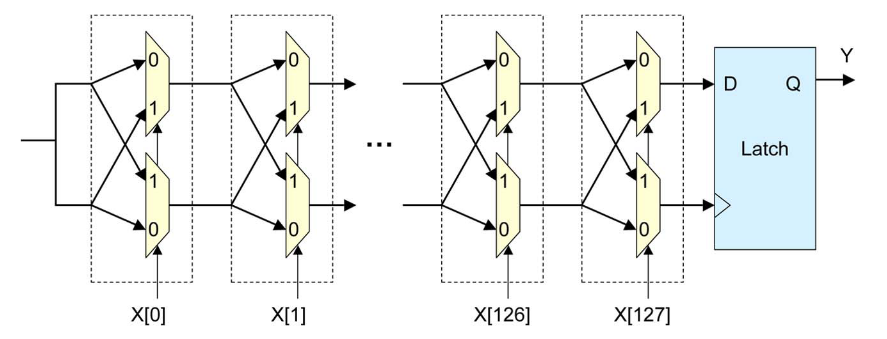
\includegraphics[width=1.0\textwidth]{arbiter_puf_circuit.png}
    \\
    Source: \cite[][p. 1130]{Herder2014}
\end{figure}

The challenge consists of $n$ bits, where $n$ is the number of switch components
in the delay line. In figure \ref{fig:arbiter_puf_circuit}, $n$ equals $128$.
Each bit configures the corresponding switch to adjust the delay path accordingly.
If a switch is set to $0$, the signals stay on their current paths,
if it is $1$, the signals cross.
At the end of the line, the latch component measures, which of the two signals arrives first.
If the paths are always symmetric regardless of switch position, a response of $0$ or $1$ is
equally likely. This would be ideal, as the variation in speed would only occur based on
variations in the manufacturing of the conductor and switches.
In practice, constructions can't always achieve exact symmetry because of space constraints. \cite[][p. 177]{Lee}

The delay of electrical components is dependant on external factors, namely
temperature, ambient noise levels and voltage variations.
The arbiter PUF solves this by not using absolute delay values, but relying on relative comparisons
between different delay characteristics. \cite[][p. 176]{Lee}

Arbiter PUFs belong to the group of fully electronic PUFs. The source of randomness is implicit, because it relies
on variations within the electrical components of the circuit, which can't be controlled in any way.
They also have internal response evaluation, which makes them intrinsic, and have a large set of \acp{CRP}
that increases exponentially while adding more switch components, making them strong PUFs. \cite[][p. 176]{Lee}


\subsubsection{SRAM PUF}

According to \cite[][p. 6]{McGrath2019}, this PUF concept was first proposed by \citeauthor*{Guajardo} in 2007 \cite{Guajardo}.
Compared to \ac{DRAM}, which is typically used as the main memory in modern computers, \ac{SRAM}
has higher power consumption and very complex internal circuitry, which makes it larger and more expensive.
However, it is still an important part in modern computers, as it allows for much lower access times than \ac{DRAM},
which makes it viable as a fast caching layer in the memory hierarchy \cite[][p. 2f]{Singh2013}.
An SRAM cache consists of peripheral circuitry which handles data input and output and address decoding.
They also consist of many SRAM cells, typically consisting of six transistors.
Each cell can hold one bit of information \cite[][p. 5]{Singh2013}.
The architecture of a typical bit cell is shown in figure \ref{fig:sram_puf_circuit}.
It consists of four load transistors $M_1 - M_4$, which store the information, two access transistors $M_5$ and $M_6$, a word line
$WL$ and the data bit-lines $BL$ and $\overline{BL}$, which carry data to and from the cell \cite[][p. 73]{Guajardo}.

The load transistors are connected in such a way, that they create a positive feedback loop.
If the voltage at node $Q$ tends towards being high, the feedback loop will amplify this tendency
and force the voltage to high. $Q$ and $\overline{Q}$ always have opposite states.
The voltage at node $Q$ dictates the bit of information stored within the cell. If $Q$ is high, the cell is $1$,
if it's low, the cell is $0$. \cite[][p. 31]{Singh2013}

\begin{figure}[H]
    \centering
    \caption{Circuit Diagram of SRAM PUF}
    \label{fig:sram_puf_circuit}
    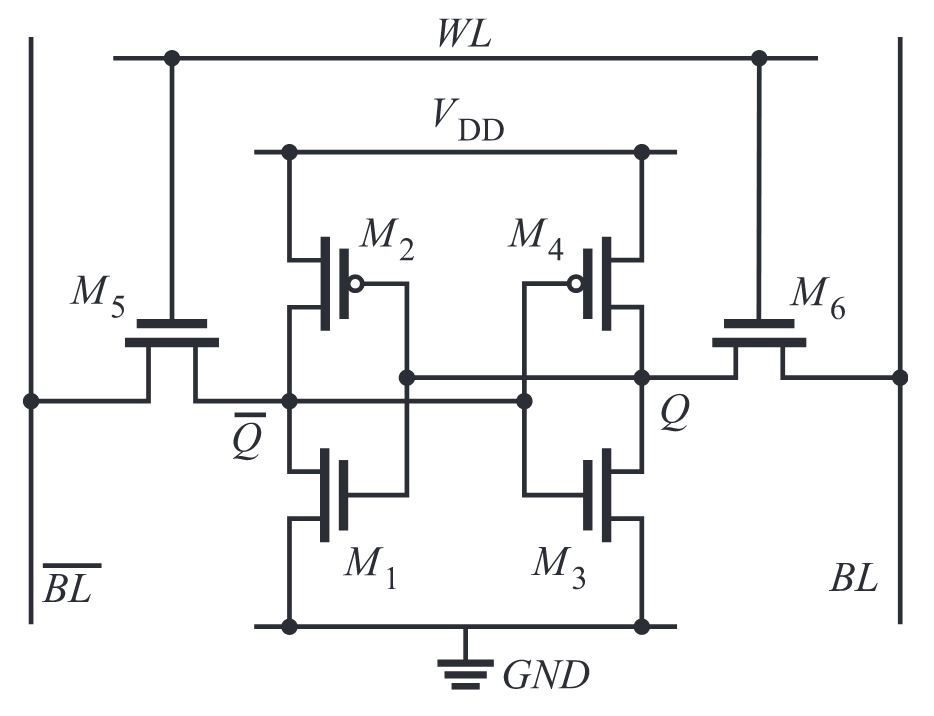
\includegraphics[width=0.6\textwidth]{sram_puf_diagram.png}
    \\
    Source: \cite[][p. 12]{McGrath2019}
\end{figure}

An SRAM cell can have three possible states:

\begin{itemize}
    \item \emph{Standby}: Here the word-line $WL$ is low, which disconnects the load transistors from the
          bit line. This means, that their state will not change as long as the load transistors are powered. \cite[][p. 31]{Singh2013}
    \item \emph{Reading}: Here, both bit-lines are set high. Then the access transistors are engaged,
          which connects the bit-lines to the load transistors. If the cell's state is $1$, $\overline{BL}$ will
          drop in voltage. If the state is $0$, $BL$ will drop in voltage. A sense amplifier measures, which of
          the bit-lines had a voltage drop and has thus read the cell.
          In the end, the word-line is set high again, to disconnect the cell \cite[][p. 32]{Singh2013}.
    \item \emph{Writing}: If a $1$ should be written, first $BL$ is set to $1$ and $\overline{BL}$ is set to $0$.
          $WL$ is set high to connect the cell to the bit-lines. Because the load transistors are much weaker
          than the bit-line drivers, they take the value of $BL$. The word-line is then disengaged\cite[][p. 36]{Singh2013}.
\end{itemize}

As SRAM cells have been scaled down to increase speed and size,
electrical deviations on an atomic-level become a challenge \cite[][p. 658]{Bhavnagarwala2001}.
The write process requires load-transistors in the cell to be relatively weak, so they can be overwritten by the voltage
one the bit-lines. This is why they are particularly vulnerable to fluctuations on an atomic level.
These variations can not be controlled during the manufacturing process, which makes them implicit \cite[][p. 73]{Guajardo}.
Under normal operation, the cells are manufactured in a way, that these fluctuations don't decrease the stability
of the cell during reads, writes and standby, in a meaningful way.
However, when powering up the SRAM, for a short period of time, the cell is not exposed to any external
electrical signal. During this time, the intrinsic electrical variations tend to a $0$ or a $1$.
This tendency is amplified due to the positive feedback loop of the load-transistor circuit.
Although the variations across multiple cells are random, they are consistent over time.
This means that a single cell will assume the same state after each power-up with a high probability,
independent from neighboring cells. \cite[][p. 73]{Guajardo}

These intrinsic variations across cells, which are stable over time, are used as the PUF.
The challenge dictates a range of cells within the SRAM cache to be read.
Because of error correction, 4600 SRAM cells are required to extract a stable 128-bit response from the PUF.
The response does not need to be converted or quantized further, as it is already in the form of binary data.
Using a 512 kbit SRAM module, a total of $512.000 / 4600 ~= 111$ \acp{CRP} is available.
This increases with the number of cells or by decreasing the secret size. \cite[][p. 73]{Guajardo}


%\subsection{Common Attacks on PUFs}

% NECESSARY EXPLANATIONS:
% Recording CRPs (sources in Majzoobi2012)
% Machine learning attacks (sources in Majzoobi2012)

% Additional possible attacks to explain
% \cite[][p.86f]{Ruehrmair2010}
% \cite[]{Gao2020} % Challenges, attacks and countermeasures
% \cite{Merli2012} % Invasive and semi-invasive, side-channel, modelling attacks
% \cite{Katzenbeisser2012} % How secure are PUFs in practice
% \cite{Ruhrmair2014} % Attacks on Weak and strong PUFs
% Tampering (Obermaier 2018)

\subsection{PUF-based Authentication}
\label{sec:puf_authentication}

This section describes the basic principles behind authentication and gives an overview of how PUFs
are used for entity authentication.

\subsubsection{Fundamentals of Authentication}

Authentication is used to establish the identity of an entity, such as a person or object.
When a person is trying to authenticate themselves, they have to prove in some way that they are
who they say they are. This can be done in three main ways \cite[][p.398]{Basavala2012}:

\begin{enumerate}
    \item By providing a secret that only they know, such as a password.
    \item By providing something only they have, such as a physical key.
    \item By using some unique physical characteristic, such as a fingerprint.
\end{enumerate}

In addition to proving the entity's identity, the authentication process also needs to reveal that the entity
was actively present and involved in the process \cite[][p. 117f]{Maes2013}.
As discussed in section \ref{sec:puf_def_of_terms}, PUFs can be closely compared to human fingerprints, as both are unclonable,
inherent and instance-specific. They therefore provide an entity-specific feature, which can be used for entity authentication.

To put it concisely, \citeauthor*{Maes2013} presents the following definition for entity authentication:

\begin{quote}
    \emph{"An entity authentication technique assures one party, through acquisition of
        corroborative evidence, of both: (i) the identity of a second party involved,
        and (ii) that the second party was active at the time the evidence was created or
        acquired."} \cite[][p. 117]{Maes2013}
\end{quote}

The two parties involved in the authentication process have specific names. The party, that wants to authenticate
itself is called the \emph{prover}, because it is proving its identity. The party it is authenticating to is
called the \emph{verifier}, because it verifies the proof of identity provided by the authenticating party. \cite[][p. 129]{Maes2013}

Contrary to authentication, authorization determines whether someone is allowed to access
a specific resource. It happens once the identity has been established and is not further considered in this thesis.

\subsubsection{Fuzzy Identification}
\label{sec:fuzzy_identification}

To authenticate an entity, it first needs to be identified.
Identification can be seen as a precondition - or a weaker form of - authentication, as the
entity merely has to provide their identity, but not prove it in a significant way or provide
evidence of its active involvement at that point in time. It is therefore sufficient in cases
where security is not important, like tracking a product in shipping.
Without clear identification, authentication does not work. \cite[][p. 118]{Maes2013}

Identification using inherent features, like the ones PUFs provide, consists of two phases \cite[][p. 119f]{Maes2013}:
\begin{enumerate}
    \item \textbf{Enrollment Phase}: Collect the inherent identities of every entity that needs to be identified.
          When using PUFs for identification, this step would involve creating \acp{CRP} and storing them in
          a database \cite{Devadas2008} or training a model, which is able to imitate the identity of the PUF.
          \cite{Majzoobi2012}
    \item \textbf{Identification Phase}: Request the entity to provide its identity and compare it to the
          set of entities collected in phase one to identify the correct entity.
          In the case of PUF-based identification, this would be requesting a response to a given challenge.
\end{enumerate}

As mentioned in section \ref{sec:intra_inter_distance}, the inherent random variations in PUFs cause responses to not
be entirely consistent, but to vary across different evaluations of the same challenge.
This presents a complication when identifying entities, as the recorded responses during the enrollment phase can be
expected to be slightly different from the responses provided during identification, which means that
a simple comparison will likely fail to identify a large amount of entities correctly. \cite[][p. 121f]{Maes2013}

The concept of identifiability was discussed in section \ref{sec:central_statistical_properties}, where it was defined
as a property found in PUFs with high probability of having a larger inter- than intra-distance.
Figure \ref{fig:inter_intra_distance_distributions} shows the distribution of the inter- and intra-distances
for a hypothetical PUF, using Hamming distances as a distance metric. \cite[][p. 121f]{Maes2013}

\begin{figure}[H]
    \centering
    \caption{Hypothetical Inter- and Intra-Distance Distributions for PUF Responses}
    \label{fig:inter_intra_distance_distributions}
    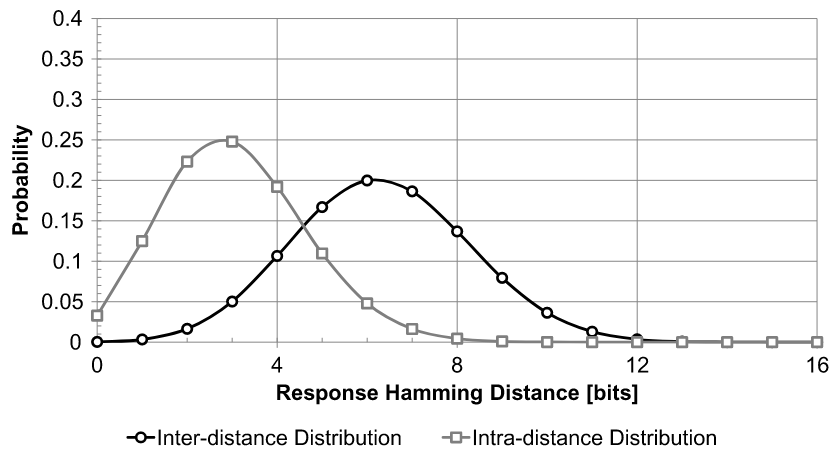
\includegraphics[width=0.7\textwidth]{inter-_intra-distance_distributions.png}
    \\
    Source: \cite[][p. 122]{Maes2013}
\end{figure}

As the inter-distance is generally larger than the intra-distance, this PUF can be considered to be identifiable.
However, there are only two assumptions, that can be made with certainty:
\begin{enumerate}
    \item Two responses with $HD = 0$ definitely stem from the same entity.
    \item Two responses with $HD > 8$ definitely stem from different entities.
\end{enumerate}

For all other distances, it is not certain wether the two responses stem from the same or different entities,
because the probability curves overlap. If there exists an overlap like this for a given PUF class,
a threshold distance $t_{id}$ needs to be defined, if it is to be used for identification.
All response pairs with a $HD$ below $t_{id}$ are considered to stem from the same instance.
All response pairs with a $HD$ above $t_{id}$ are considered to stem from different instances. \cite[][p. 121f]{Maes2013}

When identifying an entity, a CRP established during the enrollment phase is used and the response
generated during enrollment is compared to the response generated during identification.
This comparison can yield four different outcomes \cite[][p. 122f]{Maes2013}:
\begin{enumerate}
    \item \emph{True Acceptance}: The entity is the same one that was enrolled and $HD$ of both responses
          lies below $t_{id}$. The entity is correctly identified and accepted.
    \item \emph{False Acceptance}: The entity is different from the one that was enrolled and $HD$ of
          both responses lies below $t_{id}$. The entity is incorrectly identified and
          accepted.
    \item \emph{True Rejection}: The entity is different from the one that was enrolled and $HD$ of the
          responses lies above $t_{id}$. The entity is correctly rejected.
    \item \emph{False Rejection}: The entity is the same one that was enrolled, but the $HD$ of both responses
          lies above $t_{id}$. The entity is incorrectly rejected.
\end{enumerate}

The \ac{FRR} is the probability, that a given identification attempt will be falsely rejected.
It is simultaneously the probability, that the inter-distance is smaller than the identification threshold.
The \ac{FAR} is the probability, that a given identification attempt will be falsely accepted.
It is also the probability, that the intra-distance is larger than the threshold.
These metrics can be used to find the ideal threshold for the identification system \cite[][p. 123]{Maes2013}.
Figure \ref{fig:relationship_far_frr} shows the relationship between FRR and FAR for different PUF implementations.
The curves for each type show the FRR as a function of FAR.
If the threshold is lowered, the system will become more secure as the FAR decreases and the FFR increases.
If the threshold is increased (higher values for $HD$ are accepted), the system becomes more robust at the
cost of security.

\begin{figure}[H]
    \centering
    \caption{Relationship between FAR and FRR for different PUF implementations}
    \label{fig:relationship_far_frr}
    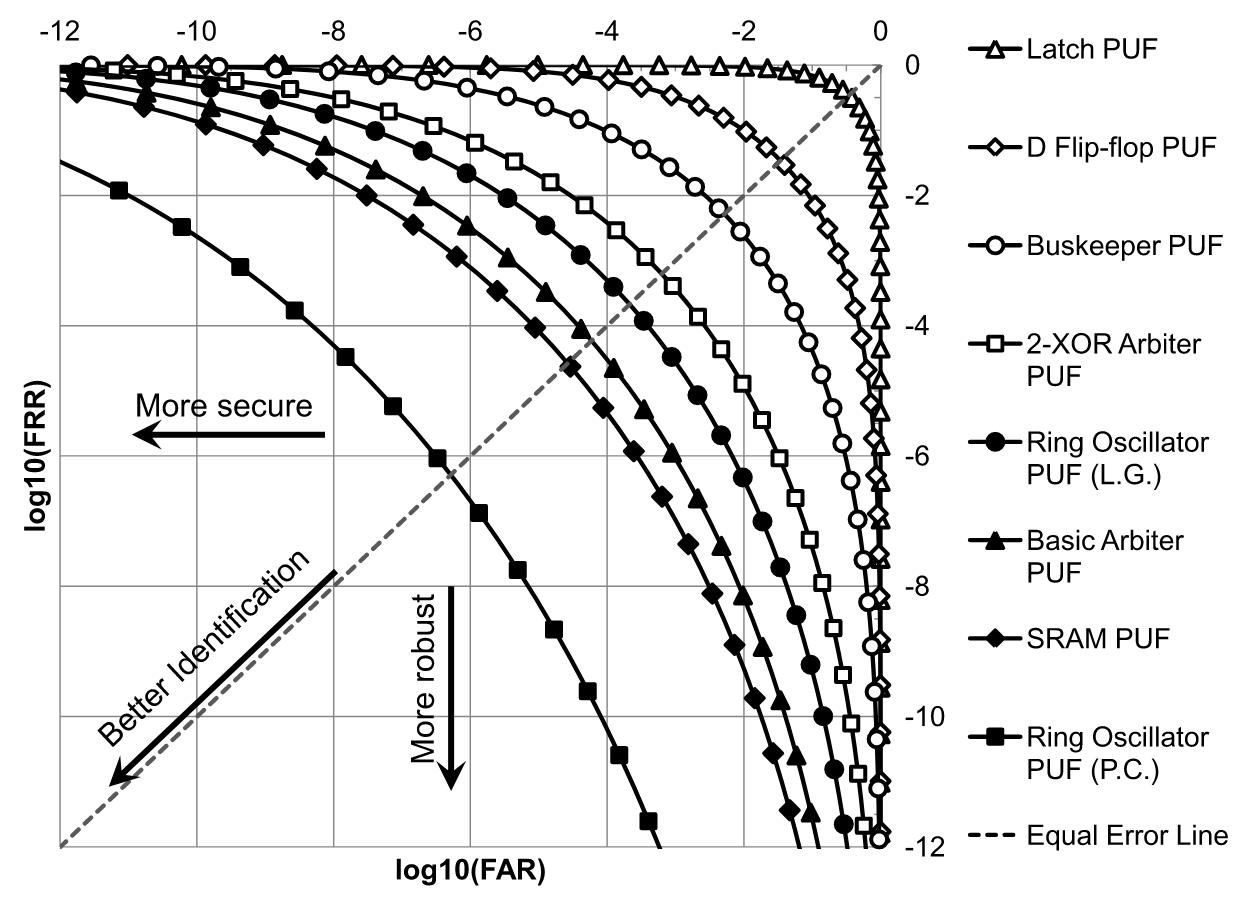
\includegraphics[width=0.7\textwidth]{relationship_far_frr.png}
    \\
    Source: \cite[][p. 125]{Maes2013}
\end{figure}

\subsubsection{Basic PUF-based Challenge-Response Authentication Protocol}
\label{sec:basic_challenge_response_protocol}

Challenge-Response protocols allow the inherent identifying features of PUFs to be used for authentication.
The most basic protocol used for PUF-based authentication is described here.

Like with identification, a challenge-response protocol using PUFs typically consists of two phases.
The first phase is \emph{enrollment}, which is identical to the first phase present in identification and
involves the verifier recording the identity of every entity by collecting many different \acp{CRP} from each
PUF and storing them in a database \cite[][p. 129f]{Maes2013}.
The verifier also assigns a unique ID to each entity and provides the entity with their ID.

\begin{figure}[h]
    \centering
    \captionsetup{justification=centering}
    \caption{UML Sequence Diagram showing the Enrollment Phase in the Basic Protocol}
    \label{fig:seq_dia_basic_protocol_enrollment}
    \begin{subfigure}{0.8\textwidth}
        \begin{plantuml}
            @startuml
            database DB as db
            participant Verifier as v
            collections "P Provers" as p
            group Enrollment Phase [for p in P where P is the number of provers]
            p -> v : Request Enrollment
            v --> p : OK
            v -> db : Create entity p
            db --> v : Entity ID for p
            loop for c in C where C is the number of CRPs
            v -> p : Send Challenge c
            p -> v : Send Response c
            v -> db : Store CRP c for ID
            db --> v : Success
            end
            v -> p : Send ID
            p --> v : OK
            end
            @enduml
        \end{plantuml}
    \end{subfigure}
    \\
    Source: Own design based on protocol proposed in \cite[][p. 129f]{Maes2013}
\end{figure}

The second phase is \emph{verification}, shown in figure \ref{fig:seq_dia_basic_protocol_verify}.
Here the authenticating entity first provides their unique ID.
The verifier looks up the available \acp{CRP} for that ID in the database and randomly selects one of them.
The respective challenge is then sent to the prover, which uses it to generate the response and sends it to
the verifier. The verifier then calculates the distance between the response recorded at enrollment
and the response received from the entity and checks, wether it is below a
previously defined authentication threshold $t_{auth}$.
If this check is successful, the entity is authenticated. The used CRP is then deleted from the database, so it
can not be used again. This protects against man-in-the-middle replay attacks \cite[][p. 130]{Maes2013}.
As previously described, there is room for error in this process, depending on how high or low $t_{auth}$ is set.

\begin{figure}[h]
    \centering
    \caption{UML Sequence Diagram showing the Verification Phase in the Basic Protocol}
    \label{fig:seq_dia_basic_protocol_verify}
    \begin{subfigure}{0.8\textwidth}
        \begin{plantuml}
            @startuml
            database DB as db
            participant Verifier as v
            entity "prover" as p
            group Verification Phase
            p -> v : Authentication Request with ID
            v --> p : OK
            v -> db : Request random CRP c
            db --> v : Send CRP c
            v -> p : Send challenge c
            p -> p : p.Eval(c)
            p -> v : Send response
            v -> v : Verify response
            alt accepted
            v -> p : Accepted
            else rejected
            v -> p : Rejected
            end
            end
            @enduml
        \end{plantuml}
    \end{subfigure}
    \\
    Source: Own design based on protocol proposed in \cite[][p. 129f]{Maes2013}
\end{figure}

\subsection{Other Applications for PUFs}
\label{sec:puf_applications}

In addition to authentication, PUFs can also be applied different scenarios.
The following is a short overview of alternative use-cases for PUFs, to get a sense of their
versatility.

\subsubsection{Storage and Generation of Cryptographic Keys}

As explained in section \ref{sec:strong_weak_pufs}, weak PUFs are not ideal for authentication, but have different uses.
One application for weak PUFs is to generate and store cryptographic keys.
The security of cryptographic protocols is entirely reliant on selecting a key with appropriate entropy
and keeping that key secret.
If an attacker were to extract the key from memory, application code or a database, the security of the given
system is compromised. \cite[][p. 3f]{McGrath2019}

By using PUFs, keys don't have to be stored permanently, but can instead be generated on demand by the PUF,
stored temporarily in memory and deleted after usage.
Essentially, the PUF itself acts as a key that only generates a copy, which is kept for a short period of time.
A challenge is sent to the PUF to generate a key (response) from it.
The response is never entirely precise, so error correction is used to ensure that keys are consistent.
Next, the response is converted into a uniform key using a hash function, which can then be used for encryption. \cite[][p. 884f]{Katzenbeisser2012}

Even though weak PUFs don't have a large set of \acp{CRP}, the central properties of PUFs are still essential.
The PUF needs to be unpredictable, so an attacker is not able to create a model
of the PUF used for key generation. If the attacker were able to do this, they could generate the appropriate
key and intercept communications.
The PUF also needs to be unclonable, so no third-party is able to have direct access to the exact \acp{CRP}.
It needs to be robust, so the same key is always generated for a given challenge. \cite[][p. 885]{Katzenbeisser2012}

\subsubsection{Object Identification}

This is again a good use-case for weak PUFs, as the burden of proving the identity is eliminated,
allowing the use of less secure constructions.
In terms of weak PUFs, identification of specific instances of a class could again be done by using a single \ac{CRP}.
After manufacturing, a generic challenge could be posed to each instance and responses could be recorded in a database.
If the identity of a device is to be established at a later point, one would simply have to issue the same challenge
to the instance and look up the response in the database \cite[][p. 118]{Maes2013}.
An example use-case for object identification would be tracking specific products in a logistics system \cite[][p. 118]{Maes2013}.
One could also use this method to detect counterfeit products, as the counterfeit would not be able to have the same
response behavior as the original, because PUFs are unclonable \cite[][p. 884]{Katzenbeisser2012}.

\subsubsection{Internet of Things}

The two applications explained above both deliver great value in the \ac{IoT} space.
As more devices and appliances in the daily life of consumers become connected and "smart",
there is a need to create trust in these devices and ensure security.
By having IoT devices generate the keys they use to authenticate to external systems using
intrinsic random variations, their identity can be reliably and consistently verified.
Constructions like the \ac{SRAM} PUF are especially interesting in this regard, as they do not require modifications
to hardware and can be applied to all classes of existing electronic devices that use embedded SRAM
memory. \cite[][p. 88]{Gao2020}
\newpage
\section{Prototype Implementation of a Protocol}
\label{sec:implementation}

\subsection{Selecting a Protocol}
\label{sec:imp_selection}

The initial plan for this thesis was to take the knowledge gained from the literature review
and use it to design a new protocol, which combines the best features of each
protocol to perfectly fit the requirements of the research project.
However, during the review it became clear, that the design of such a protocol is far
out of scope for this thesis, as extensive knowledge of cryptography and extensive
security proofs are needed to ensure the security of the protocol.
Due to this fact, the methodology is changed and one of the reviewed protocols is selected,
based on the requirements.
The protocol is then examined closely in order to fully understand it.
After that, a prototype of the infrastructure is implemented.

The goal of the research project, that this thesis is a part of, is to design a complete
authentication system, that can be used in an electronic locking system for physical access protection.
There are several criteria that can be derived from this goal:
\begin{itemize}
    \item To prevent unauthorized persons from entering protected areas, security is of the highest importance.
          The protocol should thus not be susceptible to any known attacks that could compromise the integrity of the system.
    \item The system should be practical for daily use when entering buildings, floors or rooms.
          Therefore, authentication needs to be fast, and there needs to be an easy and secure way for
          the authentication device to interface with the system.
    \item Authentication needs to be possible at multiple physical entry points
    \item Privacy and anonymity are important, because users would carry these devices
          with them for long periods of time, potentially allowing attackers to track them.
\end{itemize}

Looking at the reviewed papers in table \ref{tbl:review_results}, \cite{Gope2018}, \cite{Zhu2019} and \cite{Hristea2019} immediately
seem like good choices, because they are focused on the use-case of RFID.
This would allow the PUF devices to be embedded in RFID tags, which could interface with RFID readers
at every required physical entry point to authenticate persons against the system and grant access.
In addition, \cite{Zhu2019} delivers solid proofs for all security related features,
does not require any special PUF implementation, is able to handle noisy PUF responses
and is proven to be scalable. Therefore, this protocol is selected.

In the next section, the protocol is thoroughly examined.

\subsection{Design of the Protocol}
\label{sec:imp_design}

\subsubsection{Assumptions}

Two versions of the protocol were proposed by \citeauthor*{Zhu2019}. One version assumes an ideal PUF with
intra-distance $HD = 0$, while the other uses fuzzy extractors to deal with
noise in PUF responses \cite[][p. 6, 8]{Zhu2019}.
To keep the complexity manageable for the implementation phase, the simplified version of the protocol
is examined in this thesis. This means, that from now on, the PUF is considered to have ideal challenge-response
characteristics.
In a future work, this could easily be improved upon by implementing the enhanced version of the protocol,
which is specified in great detail in the paper \cite[][p. 8]{Zhu2019}.

Figure \ref{fig:protocol_structure} shows the layout of the underlying RFID system, including the three parties
backend server, reader and tag. The tag is a small device embedded with a PUF module, which has inherently unique
characteristics. The backend server and reader are connected through a secure channel, which an attacker
does not have access to. A physical attack on the tag is assumed to change the behavior of the PUF and make
the tag useless. Both tag and server have access to a hash function, which generates the same output for a given
input on both sides. The tag is considered to be resource limited, which means that the protocol does not specify any
spatially or computationally intensive tasks on the tag \cite[][p. 5]{Zhu2019}.

\begin{figure}[H]
    \centering
    \caption{Layout of the RFID infrastructure}
    \label{fig:protocol_structure}
    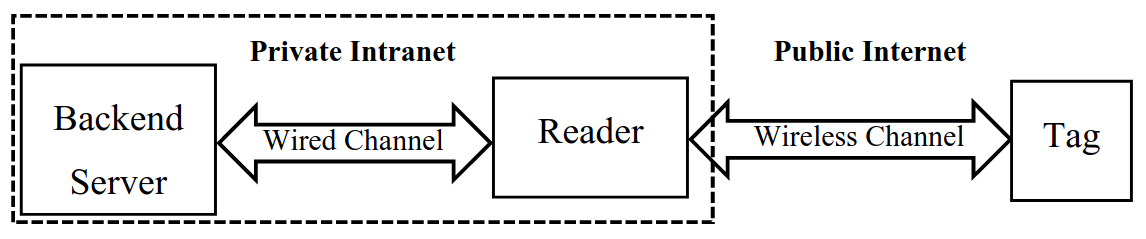
\includegraphics[width=0.7\textwidth]{structure_of_protocol.png}
    \\
    Source: \cite[][p. 5]{Zhu2019}
\end{figure}

In addition to the hash function, each party requires two more operations.
One is an XOR operation, denoted as $\oplus$, the other is a concatenation of two bitstrings, denoted as $\parallel$.

The protocol consists of two phases, the setup phase and the authentication phase. \cite[][p. 6-8]{Zhu2019}

\subsubsection{Setup Phase}

The setup phase only needs to be executed once in the beginning to initially synchronize tag and server over a
secure channel. It is comparable to the enrollment phase discussed for the basic protocol in section \ref{sec:basic_challenge_response_protocol}.
After that, the authentication phase can happen over an insecure channel \cite[][p. 7]{Zhu2019}.
Figure \ref{fig:protocol_setup} shows a sequence diagram of the setup phase.

\begin{figure}[H]
    \centering
    \caption{Setup Phase of the Proposed Protocol}
    \label{fig:protocol_setup}
    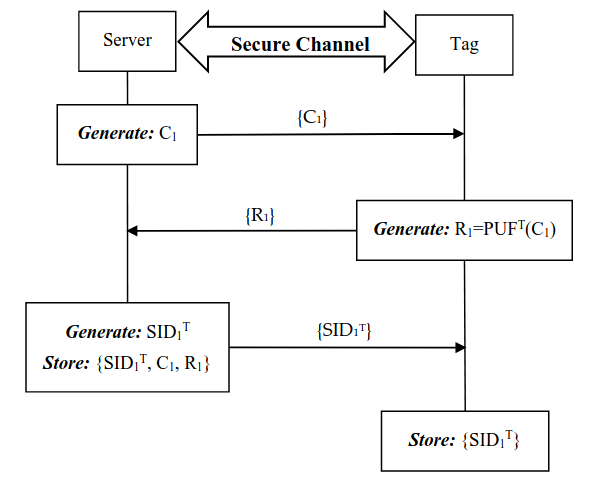
\includegraphics[width=0.7\textwidth]{setup_phase.png}
    \\
    Source: \cite[][p. 6]{Zhu2019}
\end{figure}

In the first step, the server generates a challenge and sends it to the tag.
The tag evaluates its internal PUF module using the challenge, producing a response.
The response is sent back to the server.
Next, the server prepares a unique session identity $SID$, which is used later in the first round of
authentication. The server sends it to the tag, which stores it in memory.
The server stores the $SID$, as well as the \ac{CRP} for the tag.
This concludes the setup phase. The tag is now enrolled in the system an can be used for authentication
from now on. \cite[][p. 7]{Zhu2019}

This process can be repeated for an arbitrary number of tags. The server generates a different challenge
and $SID$ for each tag and stores all of them in its database. \cite[][p. 7]{Zhu2019}

\subsubsection{Authentication Phase}

The authentication phase is described next.
Note that the reader is not shown in figure \ref{fig:protocol_authentication}, as it is connected with the server through a
secure channel. Therefore, server and reader are seen as a single unit. In reality, the messages from
the tag would be received by the reader and then forwarded to the server.
Figure \ref{fig:protocol_authentication} shows the $i$-th round of authentication.
This means that variables like $C_i$ and $R_i$ are used in the current round of authentication,
while variables like $C_{i+1}$ are prepared for the next round.

\begin{figure}[H]
    \centering
    \caption{Authentication phase of the proposed protocol}
    \label{fig:protocol_authentication}
    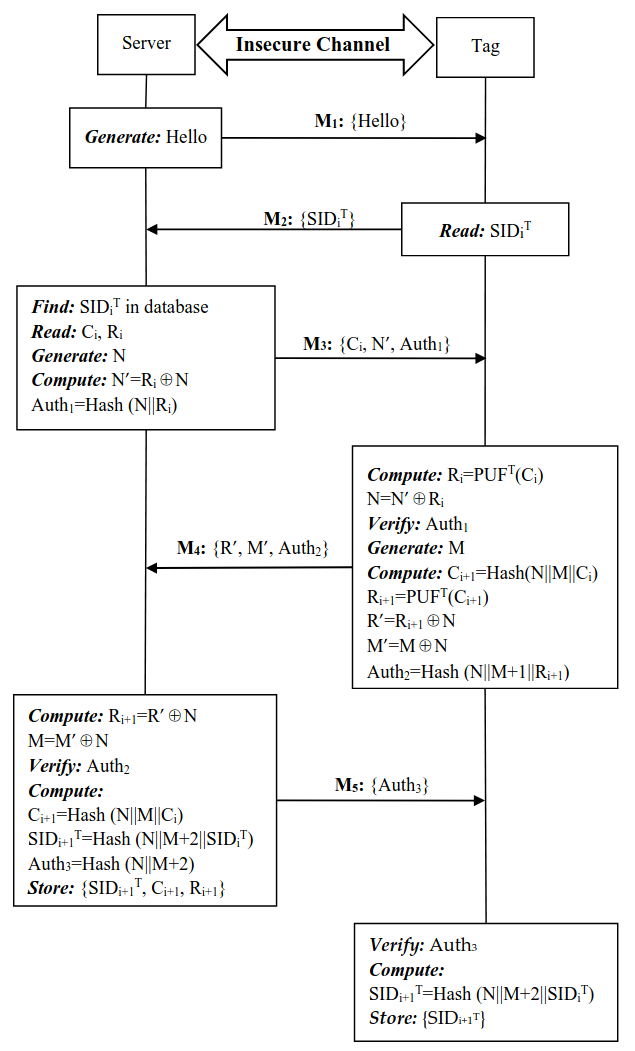
\includegraphics[width=0.7\textwidth]{authentication_phase.png}
    \\
    Source: \cite[][p. 7]{Zhu2019}
\end{figure}

In the first step, the server sends a "Hello" message to initiate the protocol. The tag answers this
with the session identifier it received during the setup phase or a previous authentication phase. \cite[][p. 7]{Zhu2019}

Next, the server uses the $SID$ to find the previously stored \ac{CRP} for that tag in the database.
If it can't find the $SID$ in the database, the tag is considered to be invalid and the authentication phase is
terminated.
Next it generates a random number $N$ and performs an XOR operation $R_i \oplus N$ on the random number and the response
to produce $N'$. It hashes a concatenation of $N$ and the response to produce $Auth_1$.
The challenge, $N'$ and $Auth_1$ are sent to the tag. \cite[][p. 7]{Zhu2019}

The tag uses the challenge $C_i$ sent by the server to evaluate its PUF module and produce
the response $R_i$. Note that in this scenario, the PUF is considered ideal, so the response is equal to the one the
server had stored in its database.
It uses the response and $N'$ to perform the same XOR operation and compute $N$.
It then produces the same hash from $N$ and the response as the server to verify $Auth_1$, as proof that
the server is genuine, because knowledge of $R_i$ is needed to calculate $Auth_1$ in the first place.
After verification, it generates a second random number $M$ and uses it to compute the next challenge $C_{i+1}$
which is a hash of the concatenation of $N$, $M$ and the challenge $C_{i+1}=Hash(N\parallel M \parallel C_i)$.
The PUF is evaluated using $C_{i+1}$ to produce the next response $R_{i+1}$.
$R'=R_{i+1} \oplus N$ and $M' = M \oplus N$ are calculated using XOR operations on $N$.
Lastly, the tag calculates $Auth_2 = Hash(N \parallel M+1 \parallel R_{i+1})$.
It sends $R'$, $M'$ and $Auth_2$ back to the server. \cite[][p. 7]{Zhu2019}

The server uses $R'$ and $M'$ received from the tag to compute $R_{i+1}$ and $M$ in the same way as the tag.
It uses them to verify $Auth_2$, which proves the identity of the tag, as the tag would not be able to generate
a correct $Auth_2$ without knowing $N$, which requires knowledge of the response to $C_i$,
that it can only know using the PUF module.
It computes the next challenge $C_{i+1}$, the next session identity $SID_{i+1}$ and $Auth_3$.
The server stores the next sid, and the next \ac{CRP} in its database and sends $Auth_3$ to the tag.
However, the old CRP and $SID$ are still kept in the database, to prevent desynchronization attacks.
The tag verifies $Auth_3$ in the same way, computes the next session ID and updates it internally. \cite[][p. 7]{Zhu2019}

If during this process, verification of any of the three $Auth$ parameters fails on either party,
the authentication procedure should be terminated to prevent attacks. If all validations pass,
each party has proven their identity to the other party. They are thus mutually authenticated. \cite[][p. 7]{Zhu2019}

\subsection{Python Implementation}
\label{sec:imp_solution}

A basic prototype of the protocol was implemented using Python.
Note that the full code is not shown in the text to improve readability and focus
on the important details. For the full implementation, refer to \ref{sec:appendix_code}.

\subsubsection{Simulating the PUF Module}

The PUF module was simulated using the \emph{pypuf} Python library \cite{pypuf}.
It provides simulations for many of the major strong PUFs, including Arbiter PUFs and Optical PUFs.
For this implementation, the \emph{ArbiterPUF} simulation was used.
The following code shows how the simulation is used in code:
\begin{lstlisting}[language=Python]
>>> from pypuf.simulation import ArbiterPUF
>>> puf = ArbiterPUF(n=64, seed=1)
>>> from pypuf.io import random_inputs
>>> puf.eval(random_inputs(n=64, N=3, seed=2))
array([ 1,  1, -1], dtype=int8)
\end{lstlisting}

The constructor takes the number of switch gates, which equals the number of challenge bits, and a seed
which defines the random characteristics of the PUF module.
The library additionally supports setting a level of noisyness for the PUF, however this was not used here.
The PUF instance provides a $puf.eval()$ method, which takes a two dimensional array of shape $(N, n)$,
where $n$ is the number of challenge bits and $N$ is the number of evaluations.
Each value of the array is an integer  of either $-1$ or $1$, which dictates wether that switch is turned on or off.
The PUF returns an array of length $N$, because on each evaluation of the PUF, a single value is returned.
The response consists of the results of $N$ evaluations, making it length $N$.

While testing, it was noticed that for small $N$, it is easy to have colliding PUF responses for different challenges,
which would decrease security of the implementation.
In the end, $N = 8; n = 64$ was used, as it proved to have no problems with value collisions, even at a high
number of evaluations.

\subsubsection{Additional Dependencies}

For hashing, the \emph{sha256} hash function from the builtin Python \emph{hashlib} was used.
The library provides a number of hash functions, which can easily be imported and used to hash different types of data.
There is no particular reasoning behind the choice of \emph{sha256} for hashing. As there are no hardware constraints
for this implementation, complexity was not an issue. However on a real RFID tag, one would not be able
to implement \emph{sha256}, as the number of logic gates required is far too high.
Therefore, in a real-world setting, a different lightweight hash function, like \emph{SPONGENT}, should be used \cite[][p. 2]{Zhu2019}.

To represent the binary challenges and responses, the Python \emph{bitstring} library was used.
It provides a \emph{BitArray} class, which allows storing binary data in a space efficient way, while also
providing methods to convert hex or integer data to binary and vice-versa, which proved useful during the
implementation of the protocol steps.
The \emph{numpy} library was used to convert the PUF responses from the \emph{ArbiterPUF} modules to and from \emph{BitArrays}.

For the creation of $SID$s, a source of randomness was needed. For this, the Python builtin \emph{uuid} module,
as well as the \emph{random} module were used.

The \emph{pytest} framework was used for testing the implementation.

\subsubsection{Structure of the Program}

The structure of the main program is shown in figure \ref{fig:implementation_structure_main}.
It consists of four main classes \emph{Server}, \emph{Tag}, \emph{TagFactory} and \emph{AuthSession}.

\begin{figure}[H]
    \centering
    \caption{UML Class Diagram showing Structure of Main Implementation}
    \label{fig:implementation_structure_main}
    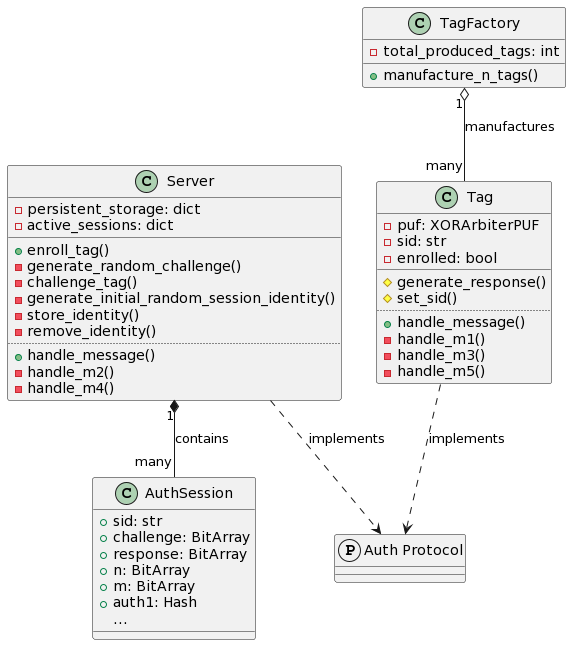
\includegraphics[width=0.7\textwidth]{implementation_structure_main.png}
\end{figure}

\emph{Server} and \emph{TagFactory} are implemented using a singleton pattern to ensure, that only one instance
can be present at all times, which helps to keep state consistent.
\emph{TagFactory} keeps track of the number of total produced \emph{Tags}, which is important for managing random variations.
As the \emph{ArbiterPUF} takes a seed integer, the factory needs to ensure, that no two tags with the same
seed are created, as they would have PUF modules with the same characteristics.
Therefore, each produced tag is assigned a different seed based on the total number of tags in existence.

The server has two types of storage, a dictionary storing active sessions of type \emph{AuthSession} and
a persistent storage dictionary, which is used for storing $SID$s and CPRs for all enrolled tags.
The server also provides an \emph{enroll\_tag} method, which takes a tag and a challenge seed and
executes the setup phase of the protocol with the tag, so it can be used for authentication in the future.
\emph{AuthSession} is a type responsible for storing all relevant data needed in the authentication phase.
The server supports the use of multiple readers at the same time, which allows multiple \emph{Tags} to be
authenticated simultaneously. Each active authentication phase needs its own \emph{AuthSession}.
The sessions are destroyed, once the tag has been authenticated and the new $SID$ and CRP have been stored
in persistent storage.

A \emph{Tag} consists of a PUF module, a variable for storing the $SID$ and a boolean which keeps track of
whether the tag has been enrolled by the server.
It also has two methods for generating responses and setting the $SID$ on the tag, which the server can call directly
during the setup phase.

Both \emph{Tag} and \emph{Server} provide a \emph{handle\_message} method.
It is used for communication between the two entities during the authentication phase.
The server \emph{handle\_message} takes an \emph{AuthMessage} , and a reader ID, which is needed to keep track of the different
simultaneous \emph{AuthSessions}. The tag's \emph{handle\_message} only takes messages, as it does not need to
keep track of sessions.

Server and Tag both implement the Auth Protocol, but this is only included in the class diagram for the purpose of
showing that both entities support the protocol. There is no specific \emph{AuthProtocol} type implemented.

In addition to the main entities described above, there is an external \emph{support} module which provides
all necessary supporting functions and constants, that are not defined by the protocol, but both parties need
to agree on.
The support module structure is shown in figure \ref{fig:implementation_structure_support}.
It includes constant values for the length of challenges and responses, as well as the hash function that
should be used by each party to verify responses.
It also provides functions for converting numpy arrays to \emph{BitArrays}, as the PUF module takes and returns
numpy arrays, but the rest of the program uses \emph{BitArrays} for handling binary data, as they
have better compatibility with hash functions and other calculations.
The basic operations required by the protocol are also provided, including creation of
a new hash, verifying a hash, XOR and concat, among others.

\begin{figure}[H]
    \centering
    \caption{UML Class Diagram of the Support Module}
    \label{fig:implementation_structure_support}
    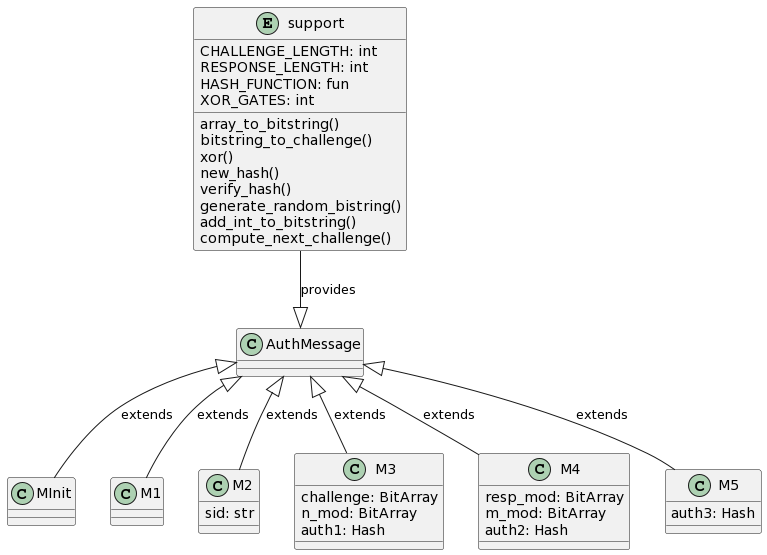
\includegraphics[width=0.8\textwidth]{implementation_structure_support.png}
\end{figure}

Lastly the \emph{support} module provides types for each of the messages required for the authentication phase.
These classes extend a common class \emph{AuthMessage} and each message holds different values, like \emph{sid}, \emph{challenge},
or \emph{auth} values, depending on what data is being sent in that step of the authentication phase.
The \emph{handle\_message} endpoint of both tag and server takes the \emph{AuthMessage} type and all of its children
and uses the specific type internally, to ensure that communication is synchronized and that
each message is handled according to protocol.

\subsubsection{Enrollment of Tags}

The following code sets up the infrastructure,
manufactures $n = 10$ tags with unique PUF modules and enrolls them with the server:

\begin{lstlisting}
factory = TagFactory()
server = Server()
n = 10
tags = factory.manufacture_n_tags(10)
for seed, tag in enumerate(tags):
    server.enroll_tag(tag, seed)
\end{lstlisting}

First, the factory and server are instantiated.
Next the factory's manufacturing method is called with the number of tags that should be created.

The code for tag creation looks like this:

\begin{lstlisting}
def manufacture_n_tags(self, n) -> List['Tag']:
    tags = []
    for i in range(0, n):
        seed = self.total_produced_tags
        puf = ArbiterPUF(n=CHALLENGE_LENGTH, seed=seed)
        tags.append(Tag(puf))
        print(f"Tag with seed {seed} manufactured")
        self.total_produced_tags += 1

    return tags
\end{lstlisting}

The seed for the PUF module is directly taken from the factories total production count.
This makes sure that each tag has a unique challenge response behavior. It also makes the behavior
of tags very predictable, but this can be ignored, because in the real world the behavior
would stem from uncontrollable intrinsic variations.
The PUF is created with the challenge length provided by the support module.
A new tag object is instantiated with the PUF module and added to the list of tags.
The list is then returned, concluding the production process.

Next, the newly created tags need to be enrolled.
Therefore, the server's enroll\_tag method is called directly for each tag.
The following code shows that method:

\begin{lstlisting}
def enroll_tag(self, tag: tag.Tag, challenge_seed: int) -> None:
    challenge = self.generate_random_challenge(challenge_seed)
    response = self.challenge_tag(tag, challenge)
    sid = self.generate_initial_random_session_identity()
    self.store_identity(sid, challenge, response)
    tag.set_sid(sid)
    print("Enrolled Tag with SID ", sid)
\end{lstlisting}

It takes the tag and a challenge seed, which it uses to generate a random challenge of the correct length.
It then calls the server's challenge\_tag method, which triggers the tag's PUF module to generate a response.
Next, a session id is generated and SID and the CRP are stored in the server's persistent storage.
Lastly, the SID is set in the tag's memory and the enrollment is finished.

\subsubsection{Authentication Phase}

To demonstrate the authentication phase, the mutual authentication of a single tag is shown here.
We assume a fully set up infrastructure with Tag \emph{tag} and Server \emph{server}.
The following code executes the authentication phase and returns a success message:

\begin{lstlisting}
tag = tags[0]
reader = 0
m1 = server.handle_message(support.MInit(), reader)
m2 = tag.handle_message(m1)
m3 = server.handle_message(m2, reader)
m4 = tag.handle_message(m3)
m5 = server.handle_message(m4, reader)
success = tag.handle_m5(m5)
if success:
    print("Tag with SID: ", tag.sid, "successfully mutually authenticated.") 
\end{lstlisting}

The server's and tag's handle\_message methods are called in an alternating way,
using the previous message returned by the other party as an argument each time.
Note that the server's method takes two arguments, to account for the use of multiple
RFID readers at the same time on a single server.
The next piece of code shows the server's handle\_message method:

\begin{lstlisting}
def handle_message(self, m: AuthMessage, reader_id: int) -> None:
    if reader_id in self.active_sessions:
        session = self.active_sessions[reader_id]
    else:
        session = self.AuthSession()
        self.active_sessions[reader_id] = session
        session.expected_message = MInit
    if type(m) != session.expected_message:
        raise TypeError(
            f"Expected {session.expected_message}, got {type(m)}")
    elif (type(m)) == MInit:
        session.expected_message = M2
        return M1()
    elif (type(m)) == M2:
        session.expected_message = M4
        return self.handle_m2(m, session)
    elif (type(m)) == M4:
        m = self.handle_m4(m, session)
        del self.active_sessions[reader_id]
    
        print(f"Tag at reader {reader_id} successfully authenticated.")
        print("New session identity written to persistent storage\n")
        return m
    else:
        raise TypeError("Unknown Message Type")

\end{lstlisting}

It first checks if there is an active session for the given reader and creates a new one if there is none.
Next it checks which type of message was sent and calls the appropriate internal method to handle
that message. To ensure consistency within a session, the last received message is recorded and
an expected\_message variable is set, which is checked before each handling call.
After handling M4, the session is deleted from the session memory, as the tag is now successfully authenticated.

The code of handle\_m2 is shown next to explain handling of specific messages:

\begin{lstlisting}
def handle_m2(self, m, session: AuthSession) -> M3:
    session.sid = m.sid
    try:
        session.challenge = self.persistent_storage[session.sid]["c"]
        session.response = self.persistent_storage[session.sid]["r"]
    except KeyError:
        raise ValueError(
            "Invalid SID sent by tag.\nTag might be invalid. Authentication terminated.")

    session.n = generate_random_bitstring(RESPONSE_LENGTH)
    session.n_mod = xor(session.response, session.n)
    session.auth1 = new_hash(
        bytes(concat(session.n, session.response).hex, 'utf-8'))
    return M3(session.challenge, session.n_mod, session.auth1)
\end{lstlisting}

M2 is sent by the tag after the initial hello message and contains the SID stored in the tag's memory.
It is stored in the session, then the persistent\_storage of the server is queried, to find the
CRP stored during enrollment or a previous authentication phase. If it is not found, the tag is assumed to
be invalid and needs to be re-enrolled.
The session generates $N$ not as an integer, but in the form of a random BitArray of length \emph{RESPONSE\_LENGTH}.
This is done so it is possible to easily perform XOR operations on the random number with the challenge.
\emph{n\_mod} represents $N'$ from the protocol definition.
\emph{auth1} is created by hashing the hexadecimal representation of the concatenation of $n$ and the $response$.
$n$, $n\_mod$ and \emph{auth1} are all stored in the session and returned in \emph{M3}.

Only a small part of this implementation has been shown in this section. To look at the full code, please reference
\ref{sec:appendix_code}.

\subsubsection{Testing the Implementation}

To test the implementation, some rudimentary test scenarios were developed using the \emph{pytest} framework.
It provides methods for asserting, wether a variable has taken on the correct value, or
if the correct errors were raised during execution.
The following tests were implemented:
\begin{itemize}
    \item Enrolling 100 tags and authenticating them in sequence.
    \item Enrolling 100 tags and authenticating them in parallel, using 100 different readers.
    \item Enrolling a single tag and authenticating it 100 times in sequence,
          to test if generation of new CRPs and SIDs works correctly.
    \item Enrolling two tags and switching them in the middle of the authentication process
          on the same reader. This should raise a ValueError, as the hashes should not be able
          to be verified.
    \item Enrolling a tag and changing its SID before the authentication phase.
          This should again lead to a ValueError, as the SID should not be found in the server's
          database.
    \item Enrolling a tag and modifying its internal PUF module before authentication.
          This would be the equivalent of an attacker tampering with the tag and changing
          the PUFs characteristics. This should raise a ValueError, as the challenge response
          behavior has changed.
\end{itemize}

As an example the last test is shown here:

\begin{lstlisting}
def test_tag_with_invalid_puf():
    """An enrolled tag with a PUF module, that was modified by an attacker,
    should not be able to authenticate."""
    factory = TagFactory()
    server = Server()
    tag = factory.manufacture_n_tags(1)[0]
    server.enroll_tag(tag, 0)

    attacker_puf = ArbiterPUF(n=CHALLENGE_LENGTH, seed=1)
    tag.puf = attacker_puf

    m1 = server.handle_message(MInit(), 0)
    m2 = tag.handle_message(m1)
    m3 = server.handle_message(m2, 0)
    with pytest.raises(ValueError):
        tag.handle_message(m3)
\end{lstlisting}

After enrollment, the puf variable of the tag is reassigned to a newly created ArbiterPUF instance
with a different seed. Following this, a ValueError is raised, because the authentication hash
can not be verified on the tag's side.
This could still be circumvented by an attacker, by disabling the tag-side hash verification,
but the tag still would not be able to generate $Auth_2$ correctly, due to
the different PUF response.

Note, that these tests do not represent a comprehensive security analysis of the protocol, but give some sense
of its capabilities. For the complete set of tests, refer to \ref{sec:appendix_code}.
\newpage
\section{Review of Existing PUF-based Authentication Protocols}
\label{sec:review}

\subsection{Methodology for the Literature Review}
\label{sec:review_methodology}

To be able to conceptualize a protocol and the surrounding infrastructure, a review of the existing literature on
\ac{PUF}-based challenge-response authentication protocols is conducted.
In \cite{Brocke2009}, \citeauthor*{Brocke2009} propose guidelines for conducting literature reviews
in the information systems field. A summary of the five-step framework can be found in \ref{sec:appendix_brocke}.

Steps one and two of the framework are not necessary in the context of a bachelor's thesis, as the scope has been
defined in section \ref{sec:introduction} and fundamentals have been laid out extensively in section \ref{sec:fundamentals}.
During the research of fundamental topics, it became clear, that defining the authentication protocol is central to answering \emph{RQ1}.
Therefore, the following search string was developed:

\begin{quote}
    \emph{(physical unclonable function OR puf OR physically unclonable function) AND (authentication OR challenge response OR challenge-response) AND (protocol)}
\end{quote}

The databases all have slightly different syntax requirements for search strings, so the actual strings used
differ a bit from this one. The exact strings are shown in \ref{sec:appendix_search_strings}.

The search string was applied to IEEEXplore, ACM and Google Scholar and restricted to document titles.
IEEExplore yielded 53 results. Most of them are centered around lightweight PUF-based authentication protocols for \ac{IoT} applications.
Results were ordered by number of citations and evaluated by their titles and abstracts.
Some articles were deemed irrelevant and thus not considered. An example for this are \cite{Zhang2021}
and \cite{Yu2022},as they propose PUF-based authentication for distributed systems using blockchain technology,
which is out of scope for this thesis.

Next the same search was conducted in the ACM Digital Library. This yielded only three results, none of which were relevant.

To fill in the gaps, the same search was conducted using Google Scholar. This yielded 104 results, most of which were
irrelevant or already contained in the IEEExplore search results.
From this search, only articles that were well-cited, very recent or offered interesting new perspectives were considered.
This resulted in eight results across different publishers, namely Elsevier, Springer and MDPI.
Backward and forward search was not used to further increase the number of papers, as the sample size was
already large enough for the purposes of this review.

\subsection{Reviewed Articles}
\label{sec:review_collected_articles}

Table \ref{tbl:review_summary} shows an overview of the papers used, source database, number of citations and year published.
As analyzing all articles in depth would be too time-consuming, a subset of the most relevant results was selected beforehand.
During this process, articles with a higher number of citations were preferred. Additionally,
because this thesis is part of a research project, concerned with creating a physical access protection system using PUF-based authentication,
literature proposed for similar purposes was preferred.
Lastly, it was important that a wide variety of approaches was included. To ensure this,
if two papers had a similar approach, the one with more citations was preferred.

\begin{table}[H]
    \centering
    \caption{Summary of reviewed papers}
    \label{tbl:review_summary}
    \begin{tabular}{|l|c|c|l|c|}
        \hline
        \textbf{Article}                                         & \textbf{Citations} & \textbf{Year} & \textbf{Database} & \textbf{Section}            \\
        \hline\hline
        \citeauthor*{Majzoobi2012} \cite{Majzoobi2012}           & 124                & 2012          & IEEExplore        & \ref{sec:review_protocol_1} \\
        \hline\citeauthor*{Gope2018} \cite{Gope2018}             & 103                & 2018          & IEEExplore        & \ref{sec:review_protocol_2} \\
        \hline\citeauthor*{Chatterjee2019} \cite{Chatterjee2019} & 95                 & 2019          & IEEExplore        & \ref{sec:review_protocol_3} \\
        \hline\citeauthor*{Braeken2018} \cite{Braeken2018}       & 78                 & 2018          & Google Scholar    & \ref{sec:review_protocol_4} \\
        \hline\citeauthor*{Bansal2020} \cite{Bansal2020}         & 48                 & 2020          & IEEExplore        & \ref{sec:review_protocol_5} \\
        \hline\citeauthor*{Zhu2019} \cite{Zhu2019}               & 19                 & 2019          & Google Scholar    & \ref{sec:review_protocol_6} \\
        \hline\citeauthor*{Jiang2019} \cite{Jiang2019}           & 10                 & 2019          & IEEExplore        & \ref{sec:review_protocol_7} \\
        \hline\citeauthor*{Gope2022} \cite{Gope2022}             & 9                  & 2022          & IEEExplore        & \ref{sec:review_protocol_8} \\
        \hline\citeauthor*{Hristea2019} \cite{Hristea2019}       & 4                  & 2019          & Google Scholar    & \ref{sec:review_protocol_9} \\
        \hline
    \end{tabular}
\end{table}

\subsection{Analysis of the collected Literature}
\label{sec:review_analysis}

Next, each of the papers is analyzed.
The focus of analysis was put on a couple of central questions:
\begin{itemize}
    \item What is the goal of the protocol and what problem does it solve?
    \item What requirements to the underlying infrastructure (hardware, databases) does the protocol have?
    \item What kinds of attacks does the protocol aim to prevent?
    \item Is the protocol a good solution for the research questions posed in section \ref{sec:research_questions}
\end{itemize}

\subsubsection{Slender PUF Protocol by \citeauthor*{Majzoobi2012}}
\label{sec:review_protocol_1}

This protocol requires the use of a PUF with a specific statistical property called the
strict PUF avalanche criterion.
It describes PUFs, which behave in a way, that any bit-flip in the challenge will result in half of
the response bits to flip. To achieve this, the protocol uses a PUF consisting of eight individual
Arbiter PUFs connected through XOR logic gates, which improves the statistical properties to fulfill
this criterion. \cite{Majzoobi2012}

As a strong PUF, it has an exponentially large set of CRPs, which limits attacks by recording previously
used \acp{CRP} (replay attacks), because the same challenge does not have to be used multiple times.
This method is also used in the basic authentication protocol discussed in section \ref{sec:basic_challenge_response_protocol}, where
CRPs are deleted from the database after usage.
This safeguard alone does not protect against machine learning attacks, where an untrusted third-party
can use previously recorded CRPs to train a model of the PUF. This model learns the response behavior
and potentially allows an attacker to calculate the appropriate response to a future challenge.
This protocol aims to make this kind of attack impossible \cite[][p. 34f]{Majzoobi2012}.

The protocol assumes that the verifier knows the relationship of challenges and responses for each
instance through a compact model of the PUF, which has been trained during the enrollment phase
and is stored in a database on the verifiers side. The model can be trained with as many CRPs as necessary,
because the PUF can be directly evaluated. After enrollment, the physical access points
that allow direct evaluation, need to be disabled to prevent potential attackers with physical access
from evaluating the PUF directly and and building a model. This is done by blowing a fuse to disable the
external pins used for access to the PUF. After this, the PUF can only be accessed through a controller on the
device, which adheres to the protocol specifications and prevents direct readouts.
The only other way to obtain knowledge about the challenge-response behavior
at this point would be by opening the PUF, which would likely change its characteristics. \cite{Majzoobi2012}

In the paper, three types of attacks on this protocol are discussed.
The first is a PUF modeling attack, where an attacker trains a model on previously
recorded CRPs to try and imitate a PUF instance. The basic PUF authentication protocol
does not protect against this kind of attack, as the full challenges and responses are
exposed during the authentication process. This protocol mitigates this risk, by not directly
exposing responses. Instead, only substrings with a random starting index are exposed.
There is still a way for an attacker to create a model by guessing the substring each time,
but the amount of CRPs required to successfully build a model increases dramatically
which greatly reduces the risk. Of course, this attack vector would have to be analyzed
much more closely before deploying a system using this protocol. \cite{Majzoobi2012}

The second is a random guessing attack.
The paper gives concrete figures for the probability of such an attack being successful.
For example, a protocol implementation with a response length of 1024 bits, substring length of 256
bits and Hamming authentication threshold of 76 would only give a $10^-11$ chance of a successful guess. \cite{Majzoobi2012}

The paper also discuss attacks that compromise the randomness of the seed by impersonating
either verifier or prover, but these are deemed to be fixable depending on the implementation. \cite{Majzoobi2012}

The main benefits of this protocol include the resiliency against ML attacks, the robustness
against noise in PUF responses without the need for traditional expensive error correction. \cite{Majzoobi2012}

\subsubsection{Lightweight Anonymous Protocol for RFID Systems by \citeauthor*{Gope2018}}
\label{sec:review_protocol_2}

This protocol was developed for using PUFs as a cryptographic primitive for
entity authentication in IoT using RFID technology.
A typical RFID system involves an RFID tag, a reader and a backend server.
The protocol requires the tag to consist of a micro controller and a tamper-proof PUF with
intrinsic random variations. It also assumes a secure connection between the reader and the backend. \cite{Gope2018}

There are many security issues and attack vectors with traditional RFID systems.
One problem with typical RFID tags is, that they threaten the user's privacy,
because identifying information stored on the tag can be retrieved without immediate
access to the device and without need for authentication by the other party.
This allows tracking the location of users.
Attacks against forward secrecy are another problem. As the communication channel in RFID
is insecure, an eavesdropper can record all traffic, although it is usually encrypted.
If at some point in the future, the encryption is broken, all previously recorded communication
can now be accessed by the attacker.
Another problem is a desynchronization attack, where a third party blocks messages between
reader and tag, to desynchronize communication. In many classical RFID authentication protocols,
the secret is exchanged frequently to provide forward secrecy. If an attacker blocks the acknowledgement
from the server, that the secret was successfully changed, the tag does not know which secret to use.
This will cause a denial of service for that tag.
Additional attacks include impersonation attacks, physical attacks, where information is retrieved
by reading the physical memory on the tag, or cloning attacks, where a copy of the tag is created. \cite{Gope2018}

This protocol aims to protect against these attacks. For example, PUFs can introduce anonymity and protect the privacy of users.
Mutual authentication between server and tag is used to protect against impersonation attacks and location tracking.
The researchers analyzed many previously proposed authentication schemes and improved upon them.
Additionally, the protocol exhibits resilience against \ac{DoS} attacks and
forward secrecy. It does not require secret keys to be stored on the tag and does not require
computationally expensive operation on the backend side, which makes it scalable. \cite{Gope2018}

\subsubsection{Protocol without explicit CRPs in Verifier Database by \citeauthor*{Chatterjee2019}}
\label{sec:review_protocol_3}

This protocol focuses on a PUF-based authentication solution for a network of distributed IoT
devices, that does not require CRPs to be stored in a database
on the verifier's side. This is important, because in all of the previously
described protocols, exposure of the database is a high security risk.
The use of \ac{IBE} and keyed hash functions allows this protocol to
only require the verifier to store a single key in its storage \cite[][p. 1f]{Chatterjee2019}.
\ac{IBE} is a type of public key encryption, where the public key can be any string \cite[][p. 8]{Chatterjee2011}.
This differs from regular \ac{PKI}, where the keys have to have a specific length and
format, dictated by the encryption system (e.g. AES). \cite[][p. 3]{Chatterjee2011}

Protecting that single key is much easier than ensuring security for an entire database.
The protocol is designed, so that a prover does not have to store a key and does not need
to do expensive computational work. The protocol allows for an unlimited number of
authentications using the same prover \cite[][p. 2f]{Chatterjee2019}.
The paper mathematically proves, that the protocol is resistant against eavesdropping attacks. \cite[][p. 8]{Chatterjee2019}

Requirements include, that each prover has to have a PUF module with intrinsic random variations
and some additional mathematical and cryptographic modules for scalar multiplication,
pairing operations and cryptographic hashing.
The verifier is required to be able to calculate a keyed hash function.  \cite[][p. 1f]{Chatterjee2019}


% If needed, this protocol can easily be described, as prosa description of steps is given on page 4


\subsubsection{Protocol for IoT by \citeauthor*{Braeken2018}}
\label{sec:review_protocol_4}

This protocol was developed for IoT applications. It aims to solve problems with a previously
published protocol and is thus developed to protect against \ac{MITM}, \ac{DoS},
impersonation and replay attacks. Additionally it offers mutual authentication, which means
that both the node and the server prove their identity to each other.
The protocol focuses on power efficiency and low computational cost \cite[][p. 1f, 8]{Braeken2018}.
It relies on storing a large amount of CRPs in a database on the verifier side and
requires a strong PUF \cite[][p. 4]{Braeken2018}.
In addition to simple authentication, it also allows the communication of two nodes
with each other, even though a central verification server is still needed. \cite[][p. 3f]{Braeken2018}

During enrollment, CRPs are shared between prover and verifier and stored in the database.
After authentication, a public and private key pair are generated. Public keys can be shared
with other nodes, with the server acting as a trusted party facilitating the exchange. \cite[][p. 4]{Braeken2018}


\subsubsection{Lightweight Protocol for V2G by \citeauthor*{Bansal2020}}
\label{sec:review_protocol_5}

This protocol is also developed for IoT applications. More specifically, it is designed to be used
in a vehicle smart grid ecosystem, which would allow to tightly integrate electric cars into the power grid
and use their batteries for energy trading and load management, enabling a more efficient use of the grid's
energy. This approach is also called \ac{V2G} and would help to manage the ever increasing power demand world
wide. However, the communication between the grid and vehicles is a privacy and security concern, because
a lot of sensitive information is exchanged between the parties, which an attacker could compromise. This
could lead to imbalanced energy transactions or privacy violations. Physical access to devices is also
easy, because vehicles are usually parked for a long time without supervision.
PUFs are used here as a means of tamper-proofing and protection against physical attacks, as no keys
need to be stored. Tampering likely changes the characteristic of the PUF and cloning is impossible. \cite[][p. 7234]{Bansal2020}

The system consists of three parties, the vehicle, an aggregator (charging station) and the power grid.
Both the aggregators and the vehicles have PUF modules, as both entities need to be authenticated
with privacy and security.
Mutual authentication is required between grid and aggregator, as well as vehicle and aggregator, to ensure
a secure exchange of encryption keys, which can be used for further communication.
To protect privacy, the keys are generated using the PUF during each authentication run and pseudonyms are used
for identifying vehicles to protect their information. \cite[][p. 7234f]{Bansal2020}
Only one challenge response pair needs to be stored on the grid server for every vehicle.
It achieves this with significantly reduced computational overhead compared to similar protocols for V2G in the field. \cite[][p. 7244]{Bansal2020}

There are four central security goals of the protocol.
Messages need to be confidential, so only authorized entities can access the information.
The integrity of messages needs to be ensured, so aggregators and the grid can know, if a message has been altered or
compromised in any way. The identity of vehicle owners has to be kept hidden from an attacker even when eavesdropping.
Mutual authentication is also a requirement to prevent impersonation attacks and false energy transfer \cite[][p. 7237]{Bansal2020}.
The paper formally proves resiliency against man-in-the-middle attacks, impersonation attacks, replay attacks and
physical attacks. It is additionally able to provide mutual authentication, protection of identity, message integrity
and security of session keys. \cite[][p. 7243]{Bansal2020}

\subsubsection{Lightweight mutual RFID protocol by \citeauthor*{Zhu2019}}
\label{sec:review_protocol_6}

This protocol is another attempt at creating a mutual authentication protocol for RFID systems.
It focuses on the same problems and goals as \cite{Gope2018}, which were discussed
in section \ref{sec:review_protocol_2}, and also makes the same assumptions about the infrastructure \cite[][p. 1, 5]{Zhu2019}.
Because the paper was published after \cite{Gope2018}, it identifies some weaknesses of that protocol and
many other proposed implementations in the RFID space and tries to improve on them.
Specifically, it identifies an issue with the protection against desynchronization attacks,
where a tag can run out of pseudo-identities that are used for authentication, if communication
is denied by an attacker too many times. This leads to the tag needing to be re-enrolled.
This protocol is able to correct that flaw. \cite[][p. 4]{Zhu2019}
Another drawback to the protocol in \cite{Gope2018} is, that it requires active RFID tags, which have an
internal power source, whereas this protocol is able to be implemented with passive tags. \cite[][p. 18]{Zhu2019}

The paper provides proofs, that the protocol is secure against a large number of attacks, including
universal untraceability of tags, ensurance of forward secrecy, secure mutual authentication,
resilience against desynchronization attacks, resiliency against physical and cloning attacks and immunity
to modeling attacks \cite[][p. 12-15]{Zhu2019}.
All of these attacks are very relevant in an RFID setting.
It is also able to do this more efficiently both in space complexity and bandwidth requirements and
comes close to other protocols in computational complexity.
The protocol is considered to be scalable. \cite[][p. 16]{Zhu2019}

\subsubsection{Two-Factor protocol by \citeauthor*{Jiang2019}}
\label{sec:review_protocol_7}

A new approach is introduced here, which has not been discussed in any other paper considered here.
This protocol combines PUF-based authentication with a password that the user enters,
to create a \ac{2FA} authentication protocol.
It is designed to be used in IoT, specifically \ac{IoV}, for managing vehicles and
automating intelligent route planing. \cite[][p. 195]{Jiang2019}

As with \cite{Bansal2020}, PUFs are a solid foundation for security in vehicles,
because they are good at preventing physical attacks, which is a big issue
with cars that are left unattended for long periods of time.
The combination with a password ensures, that a vehicle can only be authenticated if the owner
or a different trusted party is present. \cite[][p. 195]{Jiang2019}

The architecture of the protocol involves three parties, a data center which manages the information, users which
receive data from sensors and statistical data used for route planning from the data center, and the vehicle
sensors which collect real-time traffic data. It involves three phases, including system
setup, registration and login/authentication \cite[][p. 197]{Jiang2019}.
The protocol needs to be able to protect data including the vehicles
location or driving data, like speed and fuel consumption, to ensure privacy and traffic safety.
It also needs to protect against attackers injecting false information about external conditions,
threatening the safety of passengers. \cite[][p. 195f]{Jiang2019}

The paper proves that the protocol successfully implements mutual authentication, providing anonymity.
Vehicles are not identifiable or traceable, as no easily identifiable information is sent.
The protocol is secure against physical attacks because of the PUF-based nature.
The paper also claims that the protocol is secure against impersonation and desynchronization attacks,
but does not specifically argue that point.
Only one CRP per entity has to be stored by the server, which is another security benefit. \cite[][p. 199f]{Jiang2019}


\subsubsection{Protocol level approach to prevent ML attacks by \citeauthor*{Gope2022}}
\label{sec:review_protocol_8}

This protocol is aimed at IoT systems in the medical field.
The main focus is to provide a protocol which protects against machine learning attacks on PUFs.
The architecture of the systems includes several medical IoT devices like wearable health sensors or
clinical systems, which communicate with a central IoT gateway. This gateway talks to a service provider
over the internet, who provides the authentication server, information database and analysis systems.
As with many of the other papers, the wireless nature of \ac{IoMT} devices opens the system up to a
number of attacks, such as replay, man-in-the-middle, impersonation, physical and guessing attacks.
Additionally modeling attacks are a big threat. \cite[][p. 1971f]{Gope2022}

The proposed protocol aims to improve upon several previously proposed protocols including \cite{Majzoobi2012},
which is part of this review. \citeauthor*{Gope2022} criticize it, because it does not provide sufficient protection
against replay and impersonation attacks \cite[][p. 1972]{Gope2022}.
This protocol uses a special type of PUF, called \ac{OPUF}, which changes its behavior after each session,
making modelling entirely impractical.
Benefits of the protocol offer mutual authentication preserving privacy, prevention of modelling attacks,
good scalability, prevention of man-in-the-middle and replay attacks \cite[][p. 1972]{Gope2022}. It also provides forward
secrecy and prevents physical attacks. These security characteristics are argued and verified through security
simulation software \cite[][p. 1979]{Gope2022}.

\subsubsection{Destructive private mutual RFID protocol by \citeauthor*{Hristea2019}}
\label{sec:review_protocol_9}

% References 19 and 13 in this paper are concerned with comprehensive security analysis of RFID, could be interesting
% for seperate section
This protocol is another attempt at a mutual authentication protocol for RFID systems \cite[][p. 331]{Hristea2019}.
It assumes the same architecture as \cite{Zhu2019} and \cite{Gope2018}, consisting of a tag, reader and
server component. The main threats this protocol is trying to solve are impersonation and tracking
of tags. The main benefit this paper offers, is that it is stateful, meaning that it allows a
tag to have persistent state, which can be updated and shared with the reader, while also providing
resilience against physical attacks, mutual authentication and forward secrecy. \cite[][p. 332]{Hristea2019}
It is also scalable and able to prevent desynchronization attacks.
The security of the protocol is proven using a privacy model for RFID protocols. \cite[][p. 340f]{Hristea2019}

% Uses PUFs to prevent physical attacks revealing the internal secret
% Destructive privacy, no identification possible by untrusted parties due to mutual authentication

\subsection{Discussion of Results}
\label{sec:review_results}

In this section, the results of the literature review are discussed.

The methodology used for collecting the relevant literature to be reviewed is described in detail in section \ref{sec:review_methodology}.
The database queries with the respective search strings lead to a set of papers which were mostly very recent.
Almost all papers were published between 2018 and 2022, with one outlier, \cite{Majzoobi2012}, published in 2012.
An important criteria for the selection of papers was also the number of citations, as this was used as a measure of relevance
in the field. Having a lot of citations does not prove that the paper is well received, as it could also be used as a "negative example"
by other researchers. This possibility was not further investigated, and might be a weak point of this review.
Additionally, almost all papers included an extensive set of references to existing protocols, that were not found by the methodology.
This could mean, that they are either too old, did not include the relevant search terms in the title or had only few citations.

Some articles even referenced other articles that were included in the set of reviewed papers.
In \cite{Zhu2019}, \citeauthor*{Zhu2019} outlined a number of security flaws with the protocol proposed in \cite{Gope2018},
including a lack of protection against desynchronization attacks and improvements on power efficiency.
In \cite{Gope2022}, \citeauthor*{Gope2022} critized the protocol proposed by \citeauthor*{Majzoobi2012} in 2012,
mentioning its lack of protection against replay and impersonation attacks.
This again suggests, that the set of selected papers is quite relevant.

The reviewed articles provided a diverse set of different interpretations on a challenge-response protocols,
with varying requirements, intended applications, focuses and security strengths or weaknesses.

The articles focus two main application areas: RFID and IoT. IoT is further categorized in general IoT applications
\ac{IoMT} and \ac{IoV} which consists of applications for traffic management, as well as \ac{V2G}.
The varying applications lead to a number of different underlying architectures.
Protocols focused on RFID are typically based on a three layer architecture, including the RFID tags, the readers and
a backend server \cite{Gope2018} \cite{Zhu2019}.
\cite{Gope2022} provided a unique approach, where devices talk to an IoT gateway, which is connected to an external service
provider over the internet for authentication.
\ac{V2G} also has an interesting architecture, using charging stations as a communication endpoint for the IoT devices,
which then talk to a backend server.
The wide variety of devices, which can be secured with PUF, like cars, medical devices and RFID tags, also highlights the
versatility of PUF technology.

Looking at the different types of PUF required by the protocols, it is surprising to see, that many protocols don't have
a specific requirement for a PUF implementation.
This suggests, that the PUF implementation is actually not as relevant to the protocols and infrastructure as previously assumed.
Some papers on the other hand include a requirement for strong PUFs \cite{Gope2018} \cite{Zhu2019}, while others
require a certain set of statistical properties \cite{Majzoobi2012} or a specific \ac{OPUF} implementation \cite{Gope2022}.
The loose requirements of many protocols do not make the choice of PUF irrelevant. There are generally strict statistical requirements for
PUFs used in authentication, which have been touched on in section \ref{sec:fuzzy_identification}.
Some protocols only provide support for ideal PUFs which are assumed to have perfect statistical properties,
but do not actually exist in the real world. Near perfect PUF robustness can be achieved through extensive
error correction using e.g. fuzzy extractors, but this is computationally expensive. \cite{Dodis2004}

On the verifier side, there are many approaches to managing the identity of provers.
\cite{Majzoobi2012} provides the use of a lightweight model of the PUF used to verify
responses. In \cite{Zhu2019}, only one \ac{CRP} is stored in the database at any time and a new
\ac{CRP} is agreed on between prover and verifier on each authentication run.
In \cite{Chatterjee2019}, a method is proposed, that does not require the verifier to store any CRPs.

All papers strongly focus on the security aspects of their protocols, as it is crucial in providing a
secure authentication system.
Table \ref{tbl:review_results} shows an in-depth overview of the security related features of each protocol.
For interpreting these results correctly, it is important to consider, that the security of each protocol
is interpreted without extensive knowledge in the field of cyber security and cryptography.
The table should therefore not be viewed as an actual representation of the security features of each protocol,
but rather, as an overview over which features were explicitly proven to be present.
As most papers used some kind of security framework for proofs, there is a high probability, that
some of these properties were implicitly proven in a non obvious way. These kinds of proofs could not
be taken into account, which means that some protocols might actually be more secure than the table suggests.

\begin{table}[H]
    \caption{Results of the Literature Review from a Security Perspective}
    \label{tbl:review_results}
    \begin{small}
        \begin{adjustwidth}{-0.5cm}{}
            \begin{center}
                \begin{tabular}{|l|c|c|c|c|c|c|c|c|c|}
                    \hline
                    Paper                                 & \cite{Majzoobi2012}         & \cite{Gope2018}             & \cite{Chatterjee2019}       & \cite{Braeken2018}          & \cite{Bansal2020}           & \cite{Zhu2019}              & \cite{Jiang2019}            & \cite{Gope2022}             & \cite{Hristea2019}          \\
                    \hline Section                        & \ref{sec:review_protocol_1} & \ref{sec:review_protocol_2} & \ref{sec:review_protocol_3} & \ref{sec:review_protocol_4} & \ref{sec:review_protocol_5} & \ref{sec:review_protocol_6} & \ref{sec:review_protocol_7} & \ref{sec:review_protocol_8} & \ref{sec:review_protocol_9} \\
                    \hline \hline Use Case                & Any                         & RFID                        & IoT                         & IoT                         & V2G                         & RFID                        & IoV                         & IoMT                        & RFID                        \\
                    \hline Required PUF                   & Any*                        & Strong                      & Strong                      & PUF-FSM                     & N                           & Any                         & Any                         & OPUF                        & Any                         \\
                    \hline Handles Noisy PUF resp.        & \checkmark                  & \checkmark                  & \checkmark                  & \checkmark                  &                             & \checkmark                  & \checkmark                  & \checkmark                  &                             \\
                    \hline \hline Machine Learning Attack & \checkmark                  &                             &                             &                             &                             & \checkmark                  &                             & \checkmark                  &                             \\
                    \hline Random Guessing Attack         & \checkmark                  & \checkmark                  & \checkmark                  &                             &                             & \checkmark                  &                             &                             &                             \\
                    \hline Desynchronization Attack       &                             & \checkmark                  &                             &                             &                             & \checkmark                  & ?                           & \checkmark                  & \checkmark                  \\
                    \hline Denial of Service Attack       &                             & \checkmark                  &                             & \checkmark                  &                             & \checkmark                  &                             & ?                           &                             \\
                    \hline Impersonation Attack           & \checkmark                  & \checkmark                  & \checkmark                  & \checkmark                  & \checkmark                  & \checkmark                  & \checkmark                  & ?                           & \checkmark                  \\
                    \hline Physical Attack                & \checkmark                  & \checkmark                  & \checkmark                  & \checkmark                  & \checkmark                  & \checkmark                  & \checkmark                  & \checkmark                  & \checkmark                  \\
                    \hline Cloning Attack                 & \checkmark                  & \checkmark                  & \checkmark                  & \checkmark                  & \checkmark                  & \checkmark                  & \checkmark                  & \checkmark                  & \checkmark                  \\
                    \hline Mutual Authentication          &                             & \checkmark                  &                             &                             & \checkmark                  & \checkmark                  & \checkmark                  & \checkmark                  & \checkmark                  \\
                    \hline Anonymity                      &                             &                             &                             &                             & \checkmark                  & \checkmark                  & \checkmark                  & \checkmark                  & \checkmark                  \\
                    \hline Forward Secrecy                &                             & \checkmark                  &                             &                             &                             & \checkmark                  &                             & \checkmark                  & \checkmark                  \\
                    \hline Scalable                       &                             & \checkmark                  &                             &                             &                             & \checkmark                  &                             & ?                           & \checkmark                  \\
                    \hline Security Proof                 & AM                          & AM                          & AE                          & A                           & AM                          & A                           & A                           & AS                          & A                           \\
                    \hline
                \end{tabular}
            \end{center}
        \end{adjustwidth}
        \begin{flushleft}
            \vspace{0.2em}
            * PUF must fit the strict PUF avalanche criterion \newline
            \checkmark = Proven to be secure against attack or implement feature \newline
            ? = Claimed but not proven \newline
            A = Argumentative, M = Mathematical, S = Simulation, E = Experiment, N = Not specified
        \end{flushleft}
    \end{small}
\end{table}

All papers proved the security of their protocol in some way. Methods used for this include
argumentative proofs with established frameworks like Session-Key Security or the Universal Composability Framework \cite{Chatterjee2019},
mathematical proofs showing the negligible chances of a successful attack through probabilistic calculations \cite{Gope2018}, experimental
proofs using actual hardware \cite{Chatterjee2019}, or the use of software simulations \cite{Gope2022}.
An important distinguishing feature between protocols is mutual authentication.
It means, that not only the entity proves their identity to the server, but also the other way around.
This is a central requirement for privacy and anonymity, as it ensures, that entities only have to share relevant identifying
information with a party they trust. This makes it useful for preventing location tracking in RFID systems.
In regards to security, the table shows a clear winner in terms of being able to prove the most security related features,
which is \cite{Zhu2019}, published by \citeauthor*{Zhu2019} in 2019.
\newpage
\section{Prototype Implementation of a Protocol}
\label{sec:implementation}

\subsection{Selecting a Protocol}
\label{sec:imp_selection}

The initial plan for this thesis was to take the knowledge gained from the literature review
and use it to design a new protocol, which combines the best features of each
protocol to perfectly fit the requirements of the research project.
However, during the review it became clear, that the design of such a protocol is far
out of scope for this thesis, as extensive knowledge of cryptography and extensive
security proofs are needed to ensure the security of the protocol.
Due to this fact, the methodology is changed and one of the reviewed protocols is selected,
based on the requirements.
The protocol is then examined closely in order to fully understand it.
After that, a prototype of the infrastructure is implemented.

The goal of the research project, that this thesis is a part of, is to design a complete
authentication system, that can be used in an electronic locking system for physical access protection.
There are several criteria that can be derived from this goal:
\begin{itemize}
    \item To prevent unauthorized persons from entering protected areas, security is of the highest importance.
          The protocol should thus not be susceptible to any known attacks that could compromise the integrity of the system.
    \item The system should be practical for daily use when entering buildings, floors or rooms.
          Therefore, authentication needs to be fast, and there needs to be an easy and secure way for
          the authentication device to interface with the system.
    \item Authentication needs to be possible at multiple physical entry points
    \item Privacy and anonymity are important, because users would carry these devices
          with them for long periods of time, potentially allowing attackers to track them.
\end{itemize}

Looking at the reviewed papers in table \ref{tbl:review_results}, \cite{Gope2018}, \cite{Zhu2019} and \cite{Hristea2019} immediately
seem like good choices, because they are focused on the use-case of RFID.
This would allow the PUF devices to be embedded in RFID tags, which could interface with RFID readers
at every required physical entry point to authenticate persons against the system and grant access.
In addition, \cite{Zhu2019} delivers solid proofs for all security related features,
does not require any special PUF implementation, is able to handle noisy PUF responses
and is proven to be scalable. Therefore, this protocol is selected.

In the next section, the protocol is thoroughly examined.

\subsection{Design of the Protocol}
\label{sec:imp_design}

\subsubsection{Assumptions}

Two versions of the protocol were proposed by \citeauthor*{Zhu2019}. One version assumes an ideal PUF with
intra-distance $HD = 0$, while the other uses fuzzy extractors to deal with
noise in PUF responses \cite[][p. 6, 8]{Zhu2019}.
To keep the complexity manageable for the implementation phase, the simplified version of the protocol
is examined in this thesis. This means, that from now on, the PUF is considered to have ideal challenge-response
characteristics.
In a future work, this could easily be improved upon by implementing the enhanced version of the protocol,
which is specified in great detail in the paper \cite[][p. 8]{Zhu2019}.

Figure \ref{fig:protocol_structure} shows the layout of the underlying RFID system, including the three parties
backend server, reader and tag. The tag is a small device embedded with a PUF module, which has inherently unique
characteristics. The backend server and reader are connected through a secure channel, which an attacker
does not have access to. A physical attack on the tag is assumed to change the behavior of the PUF and make
the tag useless. Both tag and server have access to a hash function, which generates the same output for a given
input on both sides. The tag is considered to be resource limited, which means that the protocol does not specify any
spatially or computationally intensive tasks on the tag \cite[][p. 5]{Zhu2019}.

\begin{figure}[H]
    \centering
    \caption{Layout of the RFID infrastructure}
    \label{fig:protocol_structure}
    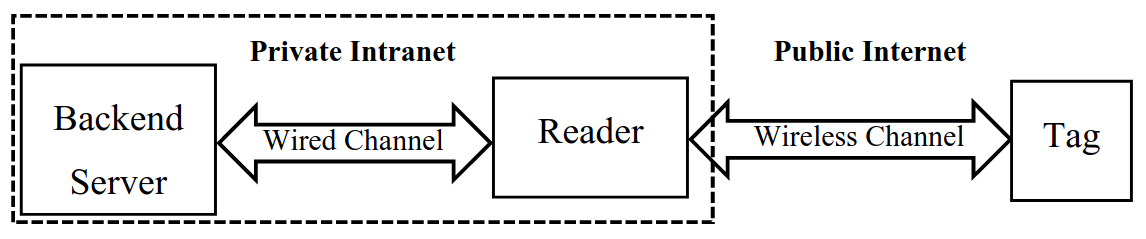
\includegraphics[width=0.7\textwidth]{structure_of_protocol.png}
    \\
    Source: \cite[][p. 5]{Zhu2019}
\end{figure}

In addition to the hash function, each party requires two more operations.
One is an XOR operation, denoted as $\oplus$, the other is a concatenation of two bitstrings, denoted as $\parallel$.

The protocol consists of two phases, the setup phase and the authentication phase. \cite[][p. 6-8]{Zhu2019}

\subsubsection{Setup Phase}

The setup phase only needs to be executed once in the beginning to initially synchronize tag and server over a
secure channel. It is comparable to the enrollment phase discussed for the basic protocol in section \ref{sec:basic_challenge_response_protocol}.
After that, the authentication phase can happen over an insecure channel \cite[][p. 7]{Zhu2019}.
Figure \ref{fig:protocol_setup} shows a sequence diagram of the setup phase.

\begin{figure}[H]
    \centering
    \caption{Setup Phase of the Proposed Protocol}
    \label{fig:protocol_setup}
    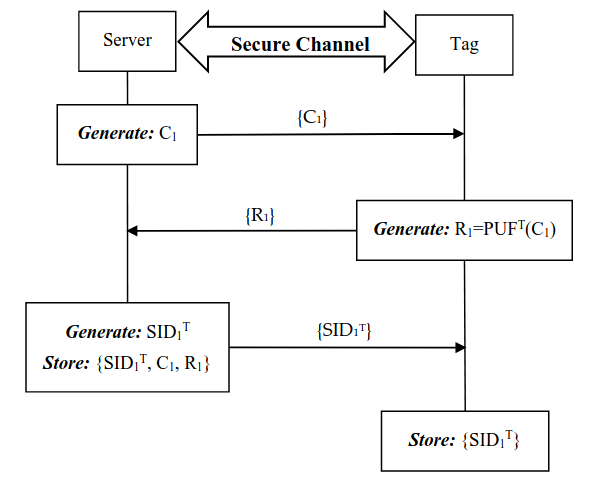
\includegraphics[width=0.7\textwidth]{setup_phase.png}
    \\
    Source: \cite[][p. 6]{Zhu2019}
\end{figure}

In the first step, the server generates a challenge and sends it to the tag.
The tag evaluates its internal PUF module using the challenge, producing a response.
The response is sent back to the server.
Next, the server prepares a unique session identity $SID$, which is used later in the first round of
authentication. The server sends it to the tag, which stores it in memory.
The server stores the $SID$, as well as the \ac{CRP} for the tag.
This concludes the setup phase. The tag is now enrolled in the system an can be used for authentication
from now on. \cite[][p. 7]{Zhu2019}

This process can be repeated for an arbitrary number of tags. The server generates a different challenge
and $SID$ for each tag and stores all of them in its database. \cite[][p. 7]{Zhu2019}

\subsubsection{Authentication Phase}

The authentication phase is described next.
Note that the reader is not shown in figure \ref{fig:protocol_authentication}, as it is connected with the server through a
secure channel. Therefore, server and reader are seen as a single unit. In reality, the messages from
the tag would be received by the reader and then forwarded to the server.
Figure \ref{fig:protocol_authentication} shows the $i$-th round of authentication.
This means that variables like $C_i$ and $R_i$ are used in the current round of authentication,
while variables like $C_{i+1}$ are prepared for the next round.

\begin{figure}[H]
    \centering
    \caption{Authentication phase of the proposed protocol}
    \label{fig:protocol_authentication}
    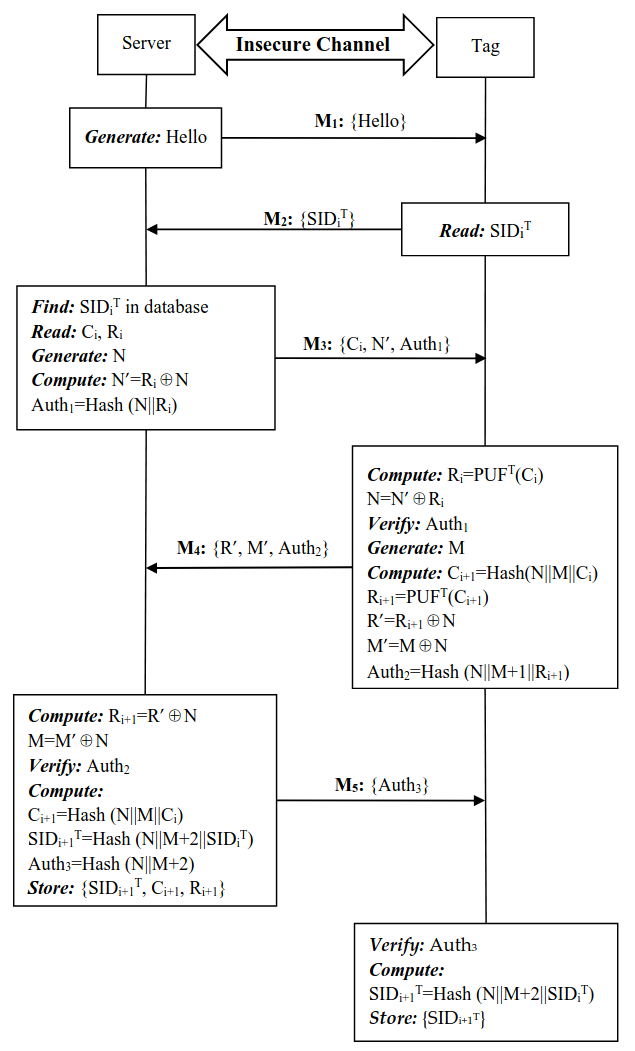
\includegraphics[width=0.7\textwidth]{authentication_phase.png}
    \\
    Source: \cite[][p. 7]{Zhu2019}
\end{figure}

In the first step, the server sends a "Hello" message to initiate the protocol. The tag answers this
with the session identifier it received during the setup phase or a previous authentication phase. \cite[][p. 7]{Zhu2019}

Next, the server uses the $SID$ to find the previously stored \ac{CRP} for that tag in the database.
If it can't find the $SID$ in the database, the tag is considered to be invalid and the authentication phase is
terminated.
Next it generates a random number $N$ and performs an XOR operation $R_i \oplus N$ on the random number and the response
to produce $N'$. It hashes a concatenation of $N$ and the response to produce $Auth_1$.
The challenge, $N'$ and $Auth_1$ are sent to the tag. \cite[][p. 7]{Zhu2019}

The tag uses the challenge $C_i$ sent by the server to evaluate its PUF module and produce
the response $R_i$. Note that in this scenario, the PUF is considered ideal, so the response is equal to the one the
server had stored in its database.
It uses the response and $N'$ to perform the same XOR operation and compute $N$.
It then produces the same hash from $N$ and the response as the server to verify $Auth_1$, as proof that
the server is genuine, because knowledge of $R_i$ is needed to calculate $Auth_1$ in the first place.
After verification, it generates a second random number $M$ and uses it to compute the next challenge $C_{i+1}$
which is a hash of the concatenation of $N$, $M$ and the challenge $C_{i+1}=Hash(N\parallel M \parallel C_i)$.
The PUF is evaluated using $C_{i+1}$ to produce the next response $R_{i+1}$.
$R'=R_{i+1} \oplus N$ and $M' = M \oplus N$ are calculated using XOR operations on $N$.
Lastly, the tag calculates $Auth_2 = Hash(N \parallel M+1 \parallel R_{i+1})$.
It sends $R'$, $M'$ and $Auth_2$ back to the server. \cite[][p. 7]{Zhu2019}

The server uses $R'$ and $M'$ received from the tag to compute $R_{i+1}$ and $M$ in the same way as the tag.
It uses them to verify $Auth_2$, which proves the identity of the tag, as the tag would not be able to generate
a correct $Auth_2$ without knowing $N$, which requires knowledge of the response to $C_i$,
that it can only know using the PUF module.
It computes the next challenge $C_{i+1}$, the next session identity $SID_{i+1}$ and $Auth_3$.
The server stores the next sid, and the next \ac{CRP} in its database and sends $Auth_3$ to the tag.
However, the old CRP and $SID$ are still kept in the database, to prevent desynchronization attacks.
The tag verifies $Auth_3$ in the same way, computes the next session ID and updates it internally. \cite[][p. 7]{Zhu2019}

If during this process, verification of any of the three $Auth$ parameters fails on either party,
the authentication procedure should be terminated to prevent attacks. If all validations pass,
each party has proven their identity to the other party. They are thus mutually authenticated. \cite[][p. 7]{Zhu2019}

\subsection{Python Implementation}
\label{sec:imp_solution}

A basic prototype of the protocol was implemented using Python.
Note that the full code is not shown in the text to improve readability and focus
on the important details. For the full implementation, refer to \ref{sec:appendix_code}.

\subsubsection{Simulating the PUF Module}

The PUF module was simulated using the \emph{pypuf} Python library \cite{pypuf}.
It provides simulations for many of the major strong PUFs, including Arbiter PUFs and Optical PUFs.
For this implementation, the \emph{ArbiterPUF} simulation was used.
The following code shows how the simulation is used in code:
\begin{lstlisting}[language=Python]
>>> from pypuf.simulation import ArbiterPUF
>>> puf = ArbiterPUF(n=64, seed=1)
>>> from pypuf.io import random_inputs
>>> puf.eval(random_inputs(n=64, N=3, seed=2))
array([ 1,  1, -1], dtype=int8)
\end{lstlisting}

The constructor takes the number of switch gates, which equals the number of challenge bits, and a seed
which defines the random characteristics of the PUF module.
The library additionally supports setting a level of noisyness for the PUF, however this was not used here.
The PUF instance provides a $puf.eval()$ method, which takes a two dimensional array of shape $(N, n)$,
where $n$ is the number of challenge bits and $N$ is the number of evaluations.
Each value of the array is an integer  of either $-1$ or $1$, which dictates wether that switch is turned on or off.
The PUF returns an array of length $N$, because on each evaluation of the PUF, a single value is returned.
The response consists of the results of $N$ evaluations, making it length $N$.

While testing, it was noticed that for small $N$, it is easy to have colliding PUF responses for different challenges,
which would decrease security of the implementation.
In the end, $N = 8; n = 64$ was used, as it proved to have no problems with value collisions, even at a high
number of evaluations.

\subsubsection{Additional Dependencies}

For hashing, the \emph{sha256} hash function from the builtin Python \emph{hashlib} was used.
The library provides a number of hash functions, which can easily be imported and used to hash different types of data.
There is no particular reasoning behind the choice of \emph{sha256} for hashing. As there are no hardware constraints
for this implementation, complexity was not an issue. However on a real RFID tag, one would not be able
to implement \emph{sha256}, as the number of logic gates required is far too high.
Therefore, in a real-world setting, a different lightweight hash function, like \emph{SPONGENT}, should be used \cite[][p. 2]{Zhu2019}.

To represent the binary challenges and responses, the Python \emph{bitstring} library was used.
It provides a \emph{BitArray} class, which allows storing binary data in a space efficient way, while also
providing methods to convert hex or integer data to binary and vice-versa, which proved useful during the
implementation of the protocol steps.
The \emph{numpy} library was used to convert the PUF responses from the \emph{ArbiterPUF} modules to and from \emph{BitArrays}.

For the creation of $SID$s, a source of randomness was needed. For this, the Python builtin \emph{uuid} module,
as well as the \emph{random} module were used.

The \emph{pytest} framework was used for testing the implementation.

\subsubsection{Structure of the Program}

The structure of the main program is shown in figure \ref{fig:implementation_structure_main}.
It consists of four main classes \emph{Server}, \emph{Tag}, \emph{TagFactory} and \emph{AuthSession}.

\begin{figure}[H]
    \centering
    \caption{UML Class Diagram showing Structure of Main Implementation}
    \label{fig:implementation_structure_main}
    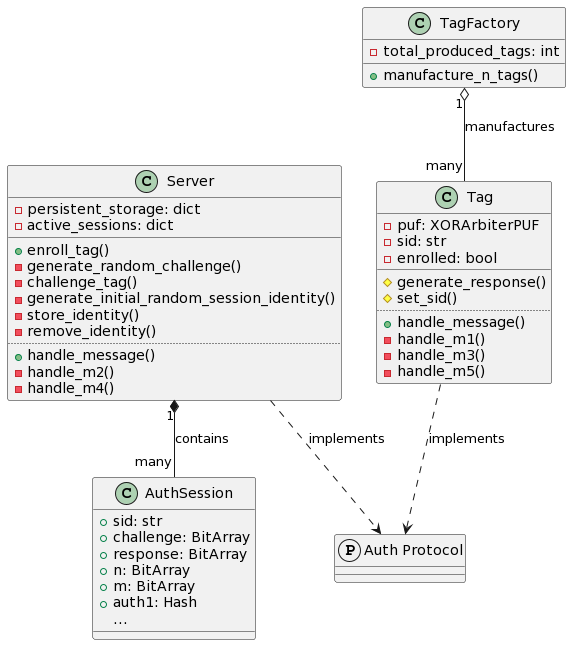
\includegraphics[width=0.7\textwidth]{implementation_structure_main.png}
\end{figure}

\emph{Server} and \emph{TagFactory} are implemented using a singleton pattern to ensure, that only one instance
can be present at all times, which helps to keep state consistent.
\emph{TagFactory} keeps track of the number of total produced \emph{Tags}, which is important for managing random variations.
As the \emph{ArbiterPUF} takes a seed integer, the factory needs to ensure, that no two tags with the same
seed are created, as they would have PUF modules with the same characteristics.
Therefore, each produced tag is assigned a different seed based on the total number of tags in existence.

The server has two types of storage, a dictionary storing active sessions of type \emph{AuthSession} and
a persistent storage dictionary, which is used for storing $SID$s and CPRs for all enrolled tags.
The server also provides an \emph{enroll\_tag} method, which takes a tag and a challenge seed and
executes the setup phase of the protocol with the tag, so it can be used for authentication in the future.
\emph{AuthSession} is a type responsible for storing all relevant data needed in the authentication phase.
The server supports the use of multiple readers at the same time, which allows multiple \emph{Tags} to be
authenticated simultaneously. Each active authentication phase needs its own \emph{AuthSession}.
The sessions are destroyed, once the tag has been authenticated and the new $SID$ and CRP have been stored
in persistent storage.

A \emph{Tag} consists of a PUF module, a variable for storing the $SID$ and a boolean which keeps track of
whether the tag has been enrolled by the server.
It also has two methods for generating responses and setting the $SID$ on the tag, which the server can call directly
during the setup phase.

Both \emph{Tag} and \emph{Server} provide a \emph{handle\_message} method.
It is used for communication between the two entities during the authentication phase.
The server \emph{handle\_message} takes an \emph{AuthMessage} , and a reader ID, which is needed to keep track of the different
simultaneous \emph{AuthSessions}. The tag's \emph{handle\_message} only takes messages, as it does not need to
keep track of sessions.

Server and Tag both implement the Auth Protocol, but this is only included in the class diagram for the purpose of
showing that both entities support the protocol. There is no specific \emph{AuthProtocol} type implemented.

In addition to the main entities described above, there is an external \emph{support} module which provides
all necessary supporting functions and constants, that are not defined by the protocol, but both parties need
to agree on.
The support module structure is shown in figure \ref{fig:implementation_structure_support}.
It includes constant values for the length of challenges and responses, as well as the hash function that
should be used by each party to verify responses.
It also provides functions for converting numpy arrays to \emph{BitArrays}, as the PUF module takes and returns
numpy arrays, but the rest of the program uses \emph{BitArrays} for handling binary data, as they
have better compatibility with hash functions and other calculations.
The basic operations required by the protocol are also provided, including creation of
a new hash, verifying a hash, XOR and concat, among others.

\begin{figure}[H]
    \centering
    \caption{UML Class Diagram of the Support Module}
    \label{fig:implementation_structure_support}
    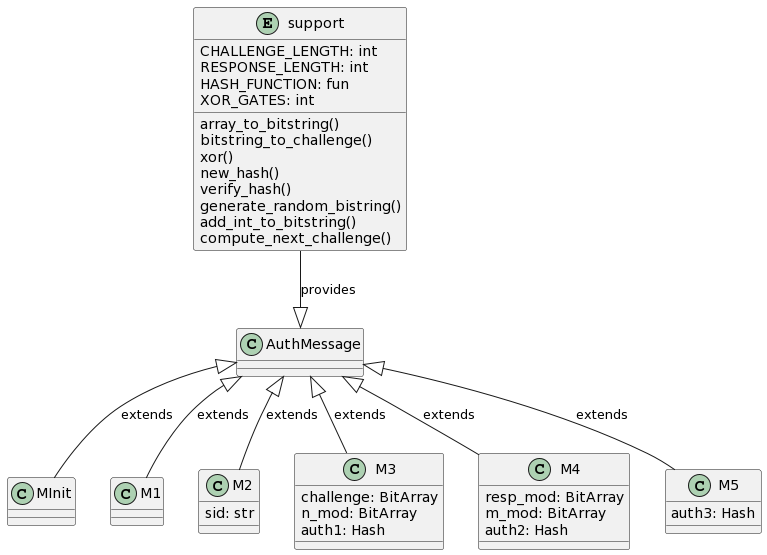
\includegraphics[width=0.8\textwidth]{implementation_structure_support.png}
\end{figure}

Lastly the \emph{support} module provides types for each of the messages required for the authentication phase.
These classes extend a common class \emph{AuthMessage} and each message holds different values, like \emph{sid}, \emph{challenge},
or \emph{auth} values, depending on what data is being sent in that step of the authentication phase.
The \emph{handle\_message} endpoint of both tag and server takes the \emph{AuthMessage} type and all of its children
and uses the specific type internally, to ensure that communication is synchronized and that
each message is handled according to protocol.

\subsubsection{Enrollment of Tags}

The following code sets up the infrastructure,
manufactures $n = 10$ tags with unique PUF modules and enrolls them with the server:

\begin{lstlisting}
factory = TagFactory()
server = Server()
n = 10
tags = factory.manufacture_n_tags(10)
for seed, tag in enumerate(tags):
    server.enroll_tag(tag, seed)
\end{lstlisting}

First, the factory and server are instantiated.
Next the factory's manufacturing method is called with the number of tags that should be created.

The code for tag creation looks like this:

\begin{lstlisting}
def manufacture_n_tags(self, n) -> List['Tag']:
    tags = []
    for i in range(0, n):
        seed = self.total_produced_tags
        puf = ArbiterPUF(n=CHALLENGE_LENGTH, seed=seed)
        tags.append(Tag(puf))
        print(f"Tag with seed {seed} manufactured")
        self.total_produced_tags += 1

    return tags
\end{lstlisting}

The seed for the PUF module is directly taken from the factories total production count.
This makes sure that each tag has a unique challenge response behavior. It also makes the behavior
of tags very predictable, but this can be ignored, because in the real world the behavior
would stem from uncontrollable intrinsic variations.
The PUF is created with the challenge length provided by the support module.
A new tag object is instantiated with the PUF module and added to the list of tags.
The list is then returned, concluding the production process.

Next, the newly created tags need to be enrolled.
Therefore, the server's enroll\_tag method is called directly for each tag.
The following code shows that method:

\begin{lstlisting}
def enroll_tag(self, tag: tag.Tag, challenge_seed: int) -> None:
    challenge = self.generate_random_challenge(challenge_seed)
    response = self.challenge_tag(tag, challenge)
    sid = self.generate_initial_random_session_identity()
    self.store_identity(sid, challenge, response)
    tag.set_sid(sid)
    print("Enrolled Tag with SID ", sid)
\end{lstlisting}

It takes the tag and a challenge seed, which it uses to generate a random challenge of the correct length.
It then calls the server's challenge\_tag method, which triggers the tag's PUF module to generate a response.
Next, a session id is generated and SID and the CRP are stored in the server's persistent storage.
Lastly, the SID is set in the tag's memory and the enrollment is finished.

\subsubsection{Authentication Phase}

To demonstrate the authentication phase, the mutual authentication of a single tag is shown here.
We assume a fully set up infrastructure with Tag \emph{tag} and Server \emph{server}.
The following code executes the authentication phase and returns a success message:

\begin{lstlisting}
tag = tags[0]
reader = 0
m1 = server.handle_message(support.MInit(), reader)
m2 = tag.handle_message(m1)
m3 = server.handle_message(m2, reader)
m4 = tag.handle_message(m3)
m5 = server.handle_message(m4, reader)
success = tag.handle_m5(m5)
if success:
    print("Tag with SID: ", tag.sid, "successfully mutually authenticated.") 
\end{lstlisting}

The server's and tag's handle\_message methods are called in an alternating way,
using the previous message returned by the other party as an argument each time.
Note that the server's method takes two arguments, to account for the use of multiple
RFID readers at the same time on a single server.
The next piece of code shows the server's handle\_message method:

\begin{lstlisting}
def handle_message(self, m: AuthMessage, reader_id: int) -> None:
    if reader_id in self.active_sessions:
        session = self.active_sessions[reader_id]
    else:
        session = self.AuthSession()
        self.active_sessions[reader_id] = session
        session.expected_message = MInit
    if type(m) != session.expected_message:
        raise TypeError(
            f"Expected {session.expected_message}, got {type(m)}")
    elif (type(m)) == MInit:
        session.expected_message = M2
        return M1()
    elif (type(m)) == M2:
        session.expected_message = M4
        return self.handle_m2(m, session)
    elif (type(m)) == M4:
        m = self.handle_m4(m, session)
        del self.active_sessions[reader_id]
    
        print(f"Tag at reader {reader_id} successfully authenticated.")
        print("New session identity written to persistent storage\n")
        return m
    else:
        raise TypeError("Unknown Message Type")

\end{lstlisting}

It first checks if there is an active session for the given reader and creates a new one if there is none.
Next it checks which type of message was sent and calls the appropriate internal method to handle
that message. To ensure consistency within a session, the last received message is recorded and
an expected\_message variable is set, which is checked before each handling call.
After handling M4, the session is deleted from the session memory, as the tag is now successfully authenticated.

The code of handle\_m2 is shown next to explain handling of specific messages:

\begin{lstlisting}
def handle_m2(self, m, session: AuthSession) -> M3:
    session.sid = m.sid
    try:
        session.challenge = self.persistent_storage[session.sid]["c"]
        session.response = self.persistent_storage[session.sid]["r"]
    except KeyError:
        raise ValueError(
            "Invalid SID sent by tag.\nTag might be invalid. Authentication terminated.")

    session.n = generate_random_bitstring(RESPONSE_LENGTH)
    session.n_mod = xor(session.response, session.n)
    session.auth1 = new_hash(
        bytes(concat(session.n, session.response).hex, 'utf-8'))
    return M3(session.challenge, session.n_mod, session.auth1)
\end{lstlisting}

M2 is sent by the tag after the initial hello message and contains the SID stored in the tag's memory.
It is stored in the session, then the persistent\_storage of the server is queried, to find the
CRP stored during enrollment or a previous authentication phase. If it is not found, the tag is assumed to
be invalid and needs to be re-enrolled.
The session generates $N$ not as an integer, but in the form of a random BitArray of length \emph{RESPONSE\_LENGTH}.
This is done so it is possible to easily perform XOR operations on the random number with the challenge.
\emph{n\_mod} represents $N'$ from the protocol definition.
\emph{auth1} is created by hashing the hexadecimal representation of the concatenation of $n$ and the $response$.
$n$, $n\_mod$ and \emph{auth1} are all stored in the session and returned in \emph{M3}.

Only a small part of this implementation has been shown in this section. To look at the full code, please reference
\ref{sec:appendix_code}.

\subsubsection{Testing the Implementation}

To test the implementation, some rudimentary test scenarios were developed using the \emph{pytest} framework.
It provides methods for asserting, wether a variable has taken on the correct value, or
if the correct errors were raised during execution.
The following tests were implemented:
\begin{itemize}
    \item Enrolling 100 tags and authenticating them in sequence.
    \item Enrolling 100 tags and authenticating them in parallel, using 100 different readers.
    \item Enrolling a single tag and authenticating it 100 times in sequence,
          to test if generation of new CRPs and SIDs works correctly.
    \item Enrolling two tags and switching them in the middle of the authentication process
          on the same reader. This should raise a ValueError, as the hashes should not be able
          to be verified.
    \item Enrolling a tag and changing its SID before the authentication phase.
          This should again lead to a ValueError, as the SID should not be found in the server's
          database.
    \item Enrolling a tag and modifying its internal PUF module before authentication.
          This would be the equivalent of an attacker tampering with the tag and changing
          the PUFs characteristics. This should raise a ValueError, as the challenge response
          behavior has changed.
\end{itemize}

As an example the last test is shown here:

\begin{lstlisting}
def test_tag_with_invalid_puf():
    """An enrolled tag with a PUF module, that was modified by an attacker,
    should not be able to authenticate."""
    factory = TagFactory()
    server = Server()
    tag = factory.manufacture_n_tags(1)[0]
    server.enroll_tag(tag, 0)

    attacker_puf = ArbiterPUF(n=CHALLENGE_LENGTH, seed=1)
    tag.puf = attacker_puf

    m1 = server.handle_message(MInit(), 0)
    m2 = tag.handle_message(m1)
    m3 = server.handle_message(m2, 0)
    with pytest.raises(ValueError):
        tag.handle_message(m3)
\end{lstlisting}

After enrollment, the puf variable of the tag is reassigned to a newly created ArbiterPUF instance
with a different seed. Following this, a ValueError is raised, because the authentication hash
can not be verified on the tag's side.
This could still be circumvented by an attacker, by disabling the tag-side hash verification,
but the tag still would not be able to generate $Auth_2$ correctly, due to
the different PUF response.

Note, that these tests do not represent a comprehensive security analysis of the protocol, but give some sense
of its capabilities. For the complete set of tests, refer to \ref{sec:appendix_code}.
\newpage
\section{Conclusion}
\label{sec:conclusion}


The thesis was able to lay a broad theoretical foundation about concepts surrounding PUFs, their types,
their implementations and PUF-based authentication.
The systematic review of the existing literature on PUF-based authentication protocols
provided an overview of the wide variety of applications, focuses, security properties
and performance factors. Through the literature review, it became clear, that the central part of any
infrastructure is the protocol, as it defines and limits the technical requirements of the underlying
hardware, backend systems and databases. Initially, it was planned to develop a new protocol fitting
the requirements of the research project. However, this goal was not realized, because the review
showed the complexity and knowledge required for designing a secure protocol goes far beyond
the scope of this thesis. A protocol fitting the requirements of the project was selected,
analyzed and a prototype was implemented.

When analyzing the methodology of the thesis critically, a couple of possible weak points can be identified.
Small parts of the fundamentals section were only based on few sources, which leaves a possibility of
incorrect and unverified information. However, the scientific quality and relevance of sources was always
ensured and no contradicting information was encountered, making this risk small.
When looking at the final selection of the protocol, it is possible, that the limited knowledge about
cryptography and security has lead to a false evaluation of certain protocols.
Additionally, the defined search string could have excluded relevant sources, opening the possibility,
that the best protocol was not found. Looking at the implementation, the security aspects
of the prototype were not closely examined.

To conclude the thesis, another look at the research questions defined in
section \ref{sec:research_questions} is necessary to evaluate the success of the thesis.
\emph{RQ1} is only partially answered by the thesis. Results almost exclusively focused on the protocol.
Other requirements for a full infrastructure, like the database implementation, the hardware required
for supporting RFID, or the requirements of access control systems, were only partially considered.

\emph{RQ2} required the implementation of a prototype and a demonstration of its
functionality. This goal was achieved as the selected protocol was implemented using
python and evaluated using a set of tests.
However, the prototype has its limitations. It has not been extensively tested
to ensure resilience against all possible types of attacks. Additionally, hardware constraints,
like a limited number of logic gates on RFID tags and the imperfect PUF responses in the real world,
have not been considered.

%-----------------------------------
% Apendix / Anhang
%-----------------------------------
\newpage
\section*{\AppendixName} %Überschrift "Anhang", ohne Nummerierung
\addcontentsline{toc}{section}{\AppendixName} %Den Anhang ohne Nummer zum Inhaltsverzeichnis hinzufügen

\begin{appendices}
    % Nachfolgende Änderungen erfolgten aufgrund von Issue 163
    \makeatletter
    \renewcommand\@seccntformat[1]{\csname the#1\endcsname:\quad}
    \makeatother
    \addtocontents{toc}{\protect\setcounter{tocdepth}{0}} %
    \renewcommand{\thesection}{\AppendixName\ \arabic{section}}
    \renewcommand\thesubsection{\AppendixName\ \arabic{section}.\arabic{subsection}}
    \section{Guidelines for Literature Reviews by \citeauthor*{Brocke2009}}
\label{sec:appendix_brocke}

This is a summary of the guidelines for literature reviews in the information systems field,
proposed by \citeauthor*{Brocke2009} in \cite{Brocke2009}.
The methodology for the literature review in this thesis is loosely based on these five-steps.

\begin{enumerate}
      \item Analyze the scope and purpose of the review by using the taxonomy on
            literature reviews proposed in \cite{Cooper1988}. This acts as a basis for further
            steps and helps to keep the review focused on a specific goal
      \item Establish concepts about the topic, that are already widely known
            and recognized in the literature. This is best done using publications like existing review articles,
            textbooks or encyclopedias.
      \item After having gained a good understanding of the concepts and fundamentals of the topic,
            search terms should be devised, that can be used for the literature searching process.
            These search terms should then be applied in the following way:
            \begin{enumerate}
                  \item Find all journals, which publish articles related to the topic.
                  \item Find all databases, which include articles from those journals.
                  \item Query these databases using keywords and search terms devised from the previously
                        acquired knowledge.
                        Estimate the relevance of articles by analyzing title, abstract, number of citations and recency.
                        Include all relevant articles in the review.
                  \item Use backward and forward search to find additional relevant literature.
            \end{enumerate}
      \item Analyze all collected literature and synthesize new knowledge from it.
            This process is enabled by using a concept matrix (proposed in \cite{Webster2002}).
            Make sure to focus on the focus and goal specified in \emph{step one}.
      \item Create a research agenda that outlines, which questions have been answered by the
            existing research and which topics future research should focus on.
\end{enumerate}

\section{Exact Search Strings used in Literature Review}
\label{sec:appendix_search_strings}

\textbf{IEEE Xplore}
\begin{quote}
      ("Document Title":physical unclonable function OR "Document Title":puf OR "Document Title":physically unclonable function) AND ("Document Title":authentication OR "Document Title":challenge response OR "Document Title":challenge-response) AND ("Document Title":protocol)
\end{quote}

\textbf{ACM Digital Library}
\begin{quote}
      [[Title: physical unclonable function] OR [Title: puf] OR [Title: physically unclonable function]] AND [[Title: authentication] OR [Title: challenge response] OR [Title: challenge-response]] AND [Title: protocol]
\end{quote}

\textbf{Google Scholar}
\begin{quote}
      intitle:protocol AND (intitle:authentication OR intitle:challenge-response OR intitle:challenge OR intitle:response) AND (intitle:puf OR intitle:physically unclonable function OR intitle:physical unclonable function)
\end{quote}


\newpage
\section{Source Code for Implementation}
\label{sec:appendix_code}
\subsection{Pipfile}
This pipfile can be used to easily set up the appropriate environment using pipenv.
\lstinputlisting{implementation/Pipfile}

\subsection{support.py}
\lstinputlisting[language=python]{implementation/support.py}

\subsection{server.py}
\lstinputlisting[language=python]{implementation/server.py}

\subsection{tag.py}
\lstinputlisting[language=python]{implementation/tag.py}

\subsection{test\_auth.py}
\lstinputlisting[language=python]{implementation/test_auth.py}
\end{appendices}
\addtocontents{toc}{\protect\setcounter{tocdepth}{2}}

%-----------------------------------
% Literaturverzeichnis
%-----------------------------------
\newpage

% Die folgende Zeile trägt ALLE Werke aus literatur.bib in das
% Literaturverzeichnis ein, egal ob sie zietiert wurden oder nicht.
% Der Befehl ist also nur zum Test der Skripte sinnvoll und muss bei echten
% Arbeiten entfernt werden.
%\nocite{*}

%\addcontentsline{toc}{section}{Literatur}

% Die folgenden beiden Befehle würden ab dem Literaturverzeichnis wieder eine
% römische Seitennummerierung nutzen.
% Das ist nach dem Leitfaden nicht zu tun. Dort steht nur dass 'sämtliche
% Verzeichnisse VOR dem Textteil' römisch zu nummerieren sind. (vgl. S. 3)
%\pagenumbering{Roman} %Zähler wieder römisch ausgeben
%\setcounter{page}{4}  %Zähler manuell hochsetzen

% Ausgabe des Literaturverzeichnisses

% Keine Trennung der Werke im Literaturverzeichnis nach ihrer Art
% (Online/nicht-Online)
%\begin{RaggedRight}
%\printbibliography
%\end{RaggedRight}

% Alternative Darstellung, die laut Leitfaden genutzt werden sollte.
% Dazu die Zeilen auskommentieren und folgenden code verwenden:

% Literaturverzeichnis getrennt nach Nicht-Online-Werken und Online-Werken
% (Internetquellen).
% Die Option nottype=online nimmt alles, was kein Online-Werk ist.
% Die Option heading=bibintoc sorgt dafür, dass das Literaturverzeichnis im
% Inhaltsverzeichnis steht.
% Es ist übrigens auch möglich mehrere type- bzw. nottype-Optionen anzugeben, um
% noch weitere Arten von Zusammenfassungen eines Literaturverzeichnisse zu
% erzeugen.
% Beispiel: [type=book,type=article]
\printbibliography[nottype=online,heading=bibintoc,title={\langde{Literaturverzeichnis}\langen{Bibliography}}]

% neue Seite für Internetquellen-Verzeichnis
\newpage

% Laut Leitfaden 2018, S. 14, Fussnote 44 stehen die Internetquellen NICHT im
% Inhaltsverzeichnis, sondern gehören zum Literaturverzeichnis.
% Die Option heading=bibintoc würde die Internetquelle als eigenen Eintrag im
% Inhaltsverzeicnis anzeigen.
%\printbibliography[type=online,heading=bibintoc,title={\headingNameInternetSources}]
\printbibliography[type=online,heading=subbibliography,title={\headingNameInternetSources}]

\newpage
\pagenumbering{gobble} % Keine Seitenzahlen mehr

%-----------------------------------
% Ehrenwörtliche Erklärung
%-----------------------------------
\section*{%
	\langde{Ehrenwörtliche Erklärung}
	\langen{Declaration in lieu of oath}}
\langde{Hiermit versichere ich, dass die vorliegende Arbeit von mir selbstständig und ohne unerlaubte Hilfe angefertigt worden ist, insbesondere dass ich alle Stellen, die wörtlich oder annähernd wörtlich aus Veröffentlichungen entnommen sind, durch Zitate als solche gekennzeichnet habe. Ich versichere auch, dass die von mir eingereichte schriftliche Version mit der digitalen Version übereinstimmt. Weiterhin erkläre ich, dass die Arbeit in gleicher oder ähnlicher Form noch keiner Prüfungsbehörde/Prüfungsstelle vorgelegen hat. Ich erkläre mich damit einverstanden, dass die Arbeit der Öffentlichkeit zugänglich gemacht wird. Ich erkläre mich damit einverstanden, dass die Digitalversion dieser Arbeit zwecks Plagiatsprüfung auf die Server externer Anbieter hochgeladen werden darf. Die Plagiatsprüfung stellt keine Zurverfügungstellung für die Öffentlichkeit dar.}
\langen{I hereby declare that I produced the submitted paper with no assistance from any other party and without the use of any unauthorized aids and, in particular, that I have marked as quotations all passages which are reproduced verbatim or near-verbatim from publications. Also, I declare that this paper has never been submitted before to any examination board in either its present form or in any other similar version. I herewith agree that this paper may be published. I herewith consent that this paper may be uploaded to the server of external contractors for the purpose of submitting it to the contractors' plagiarism detection systems. Uploading this paper for the purpose of submitting it to plagiarism detection systems is not a form of publication.}


\par\medskip
\par\medskip

\vspace{5cm}

\begin{table}[H]
	\centering
	\begin{tabular*}{\textwidth}{c @{\extracolsep{\fill}} ccccc}
		\myOrt, \the\day.\the\month.\the\year
		&
		% Hinterlege deine eingescannte Unterschrift im Verzeichnis /abbildungen und nenne sie unterschrift.png
		% Bilder mit transparentem Hintergrund können teils zu Problemen führen
		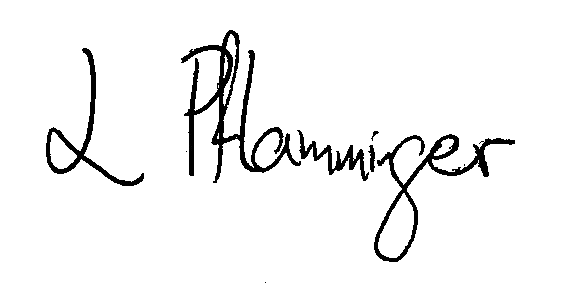
\includegraphics[width=0.35\textwidth]{unterschrift}\vspace*{-0.35cm}
		\\
		\rule[0.5ex]{12em}{0.55pt} & \rule[0.5ex]{12em}{0.55pt} \\
		\langde{(Ort, Datum)}\langen{(Location, Date)} & \langde{(Eigenhändige Unterschrift)}\langen{(handwritten signature)}
		\\
	\end{tabular*} \\
\end{table}

\end{document}
